% !TEX program = xelatex
\documentclass[11pt, UTF8, a4paper]{ctexart} % 如果内容很多，可以改为 ctexrep

% 宏包引入
\usepackage[margin=2.5cm]{geometry} % 页面边距
\usepackage{graphicx} % 插入图片
\graphicspath{{images/}}
\usepackage{amsmath, amssymb} % 数学公式（运动学、PID计算必备）
\usepackage{hyperref} % 超链接与书签
\usepackage[table]{xcolor} % 颜色支持
\usepackage{listings} % 代码块排版
\usepackage{tabularx}
\usepackage[most]{tcolorbox} % 提示框（用于写“踩坑提示”）
\usepackage{array}
\usepackage{booktabs}
\usepackage{twemojis}
\usepackage{listings}
\usepackage{menukeys}
\usepackage{float} % 强制图片位置

% 样式设置
% 超链接样式
\hypersetup{
    colorlinks=true,          % 开启链接颜色（去掉难看的方框）
    urlcolor=black,   % 网页链接的颜色（优雅的深蓝色）
    linkcolor=black,  % 内部链接（目录、章节）的颜色（黑色）
}

% 定义代码高亮使用的颜色
\definecolor{codegreen}{rgb}{0,0.6,0}
\definecolor{codegray}{rgb}{0.5,0.5,0.5}
\definecolor{codepurple}{rgb}{0.58,0,0.82}
\definecolor{backcolour}{rgb}{0.95,0.95,0.92}

% 设置代码块全局样式
\lstset{
    backgroundcolor=\color{backcolour},   % 背景色
    commentstyle=\color{codegreen},       % 注释颜色
    keywordstyle=\color{blue}\bfseries,   % 关键字颜色与加粗
    numberstyle=\tiny\color{codegray},    % 行号样式
    stringstyle=\color{codepurple},       % 字符串颜色
    basicstyle=\ttfamily\small,           % 基础字体（等宽小号）
    breakatwhitespace=false,         
    breaklines=true,                      % 自动折行（防止代码过长超出边界）
    captionpos=b,                         % 标题位置（b代表底部）
    keepspaces=true,                 
    numbers=left,                         % 行号显示在左侧
    numbersep=5pt,                  
    showspaces=false,                
    showstringspaces=false,
    showtabs=false,                  
    tabsize=4                             % Tab 宽度为 4
}

% 自定义提示框 (用于避坑指南)
\newtcolorbox{tipbox}[1][]{
    colback=blue!5!white,
    colframe=blue!75!black,
    fonttitle=\bfseries,
    title=💡 提示/避坑: #1
}

% 文档信息
\title{\textbf{Ubuntu 双系统安装教程}}
\author{安徽理工大学 RoboCup 实验室}
\date{\today}

% 页眉页脚设置
\usepackage{fancyhdr}
\pagestyle{fancy}
\fancyhf{} % 清空所有默认的页眉页脚设置
% 只设置页脚中央为页码，页眉保持空白
\cfoot{\thepage} 
% 移除页眉那条横线 (Remove the header rule line)
\renewcommand{\headrulewidth}{0pt}

% ============================正文开始==============================================
\begin{document}

\maketitle

本入门指南的源码在\url{https://github.com/LR2933/robocup-3d-getting-started}

欢迎star和pr。
\tableofcontents % 生成目录
\vspace{5cm} 
\newpage
\section{制作启动盘}
\subsection{下载Ubuntu系统镜像}
我们选择Ubuntu 24.04.4 LTS版本
\smallbreak
\url{https://releases.ubuntu.com/noble/ubuntu-24.04.4-desktop-amd64.iso}
\smallbreak
下载缓慢，建议直接群里找学长发的文件，或者问学长要。
\subsection{下载制作工具}
我们选择Rufus工具来制作启动盘。
\smallbreak
\url{https://github.com/pbatard/rufus/releases/download/v4.14/rufus-4.14.exe}
\smallbreak
\subsection{制作启动盘}
准备一个至少8GB的U盘，注意备份U盘里的数据，因为制作启动盘会格式化U盘清空U盘里的所有数据。
\smallbreak
将U盘插入电脑，打开Rufus。
\smallbreak
\textbf{设备}选择你的U盘。
\smallbreak
\textbf{引导类型选择类型}点击下面的\textbf{选择}，然后选择你下载的Ubuntu系统镜像。
\smallbreak
\textbf{分区方案}选择GPT。
\smallbreak
其他保持默认即可，然后点击开始。
\begin{figure}[H]
    \centering 
    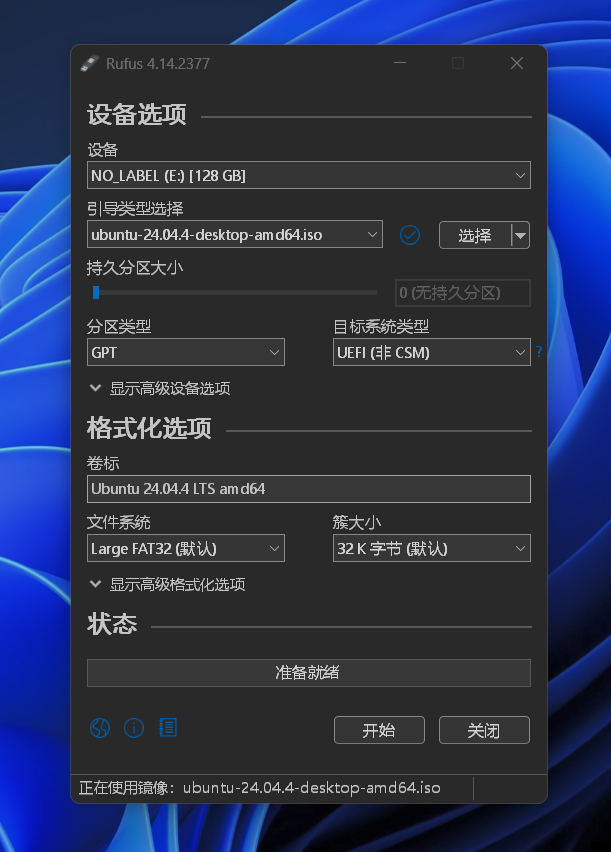
\includegraphics[width=0.5\textwidth]{rufus.png} 
\end{figure}
出现以下弹窗，选择“写入ISO映像模式（推荐）”，点击确定。如果后面的步骤电脑无法从 U 盘引导启动，可以重新制作启动盘选择“写入DD映像模式”再试试。
\begin{figure}[H]
    \centering 
    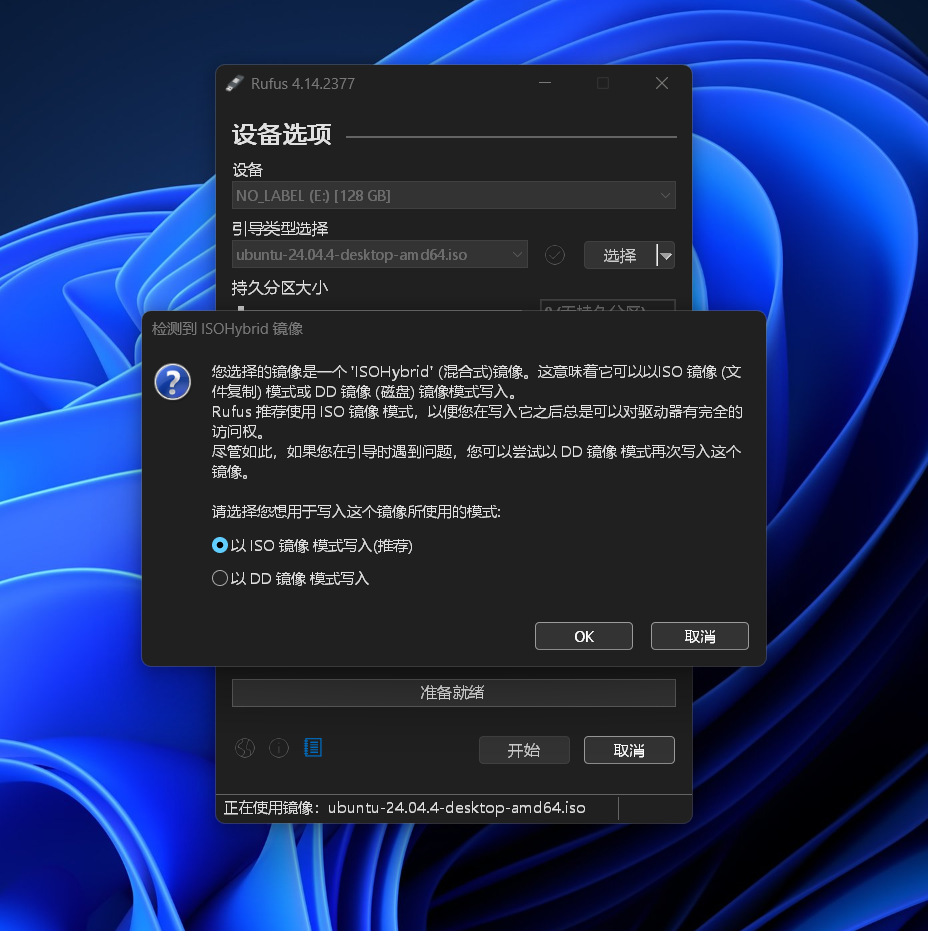
\includegraphics[width=0.5\textwidth]{rufus2.png} 
\end{figure}
如下图就是制作成功了，(如果出错了，重启rufus试试)
\begin{figure}[H]
    \centering 
    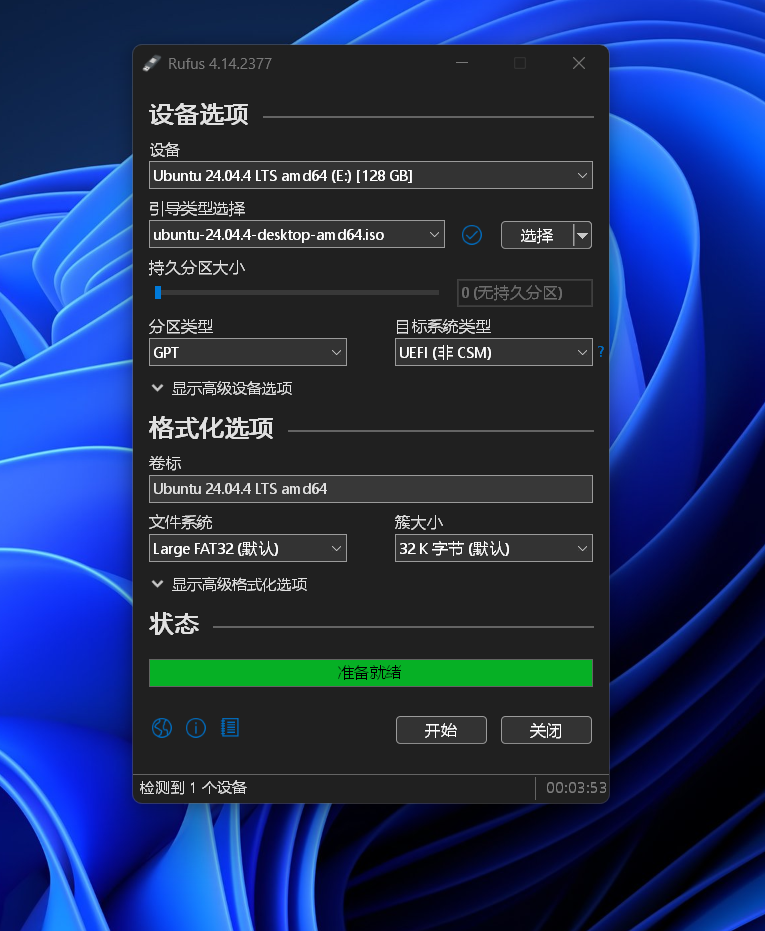
\includegraphics[width=0.5\textwidth]{rufus3.png} 
\end{figure}
\newpage

\section{给Ubuntu腾出空间}
\subsection{确认电脑还有多少剩余空间并决定分配多少给Ubuntu}
按下 \keys{\cmd + E} 打开资源管理器。(先按 \keys{\cmd} 再按 \keys{E} ，不要同时按，按 \keys{E} 的时候 \keys{\cmd} 不要松开)
\smallbreak
\begin{figure}[htbp]
    \centering 
    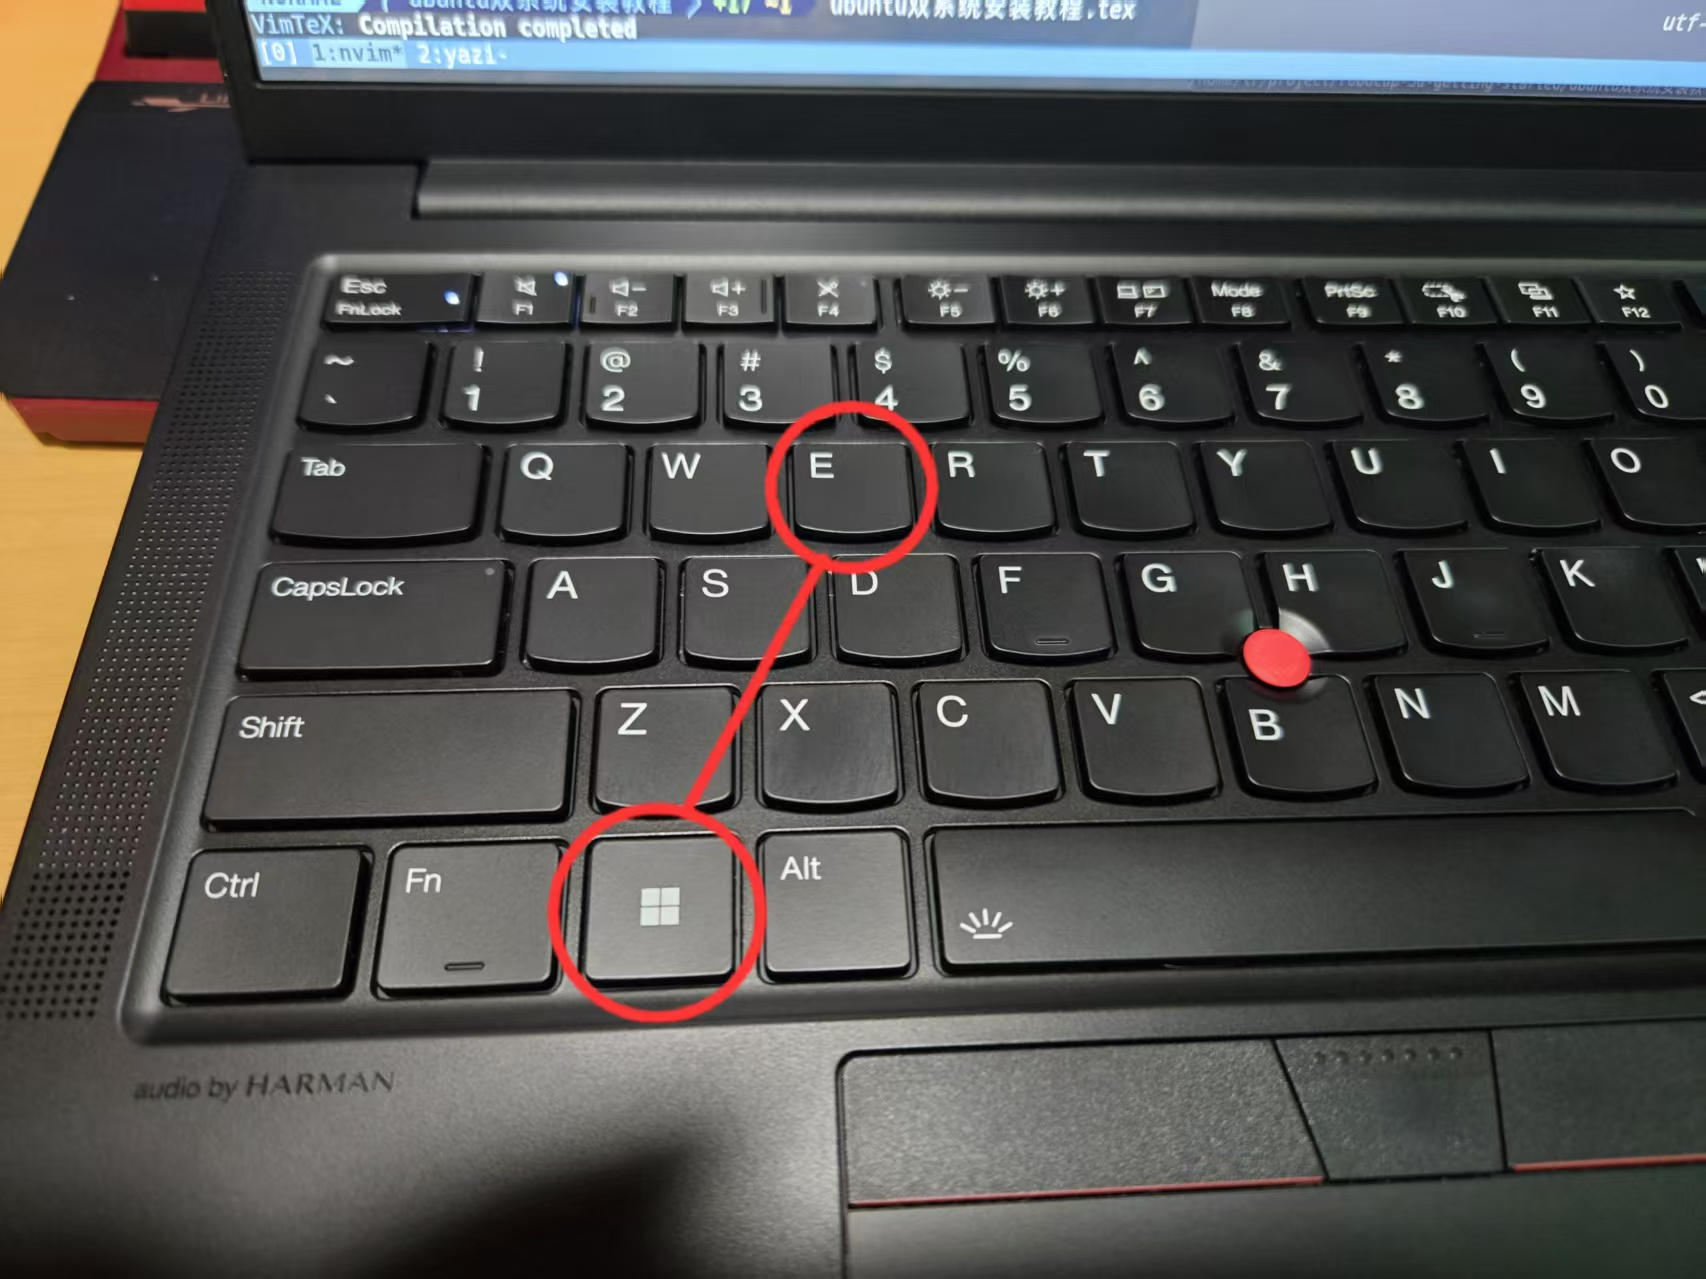
\includegraphics[width=0.5\textwidth]{3.jpg} 
\end{figure}
找到此电脑，可以查看各个盘的剩余空间。
\smallbreak
\begin{figure}[htbp]
    \centering 
    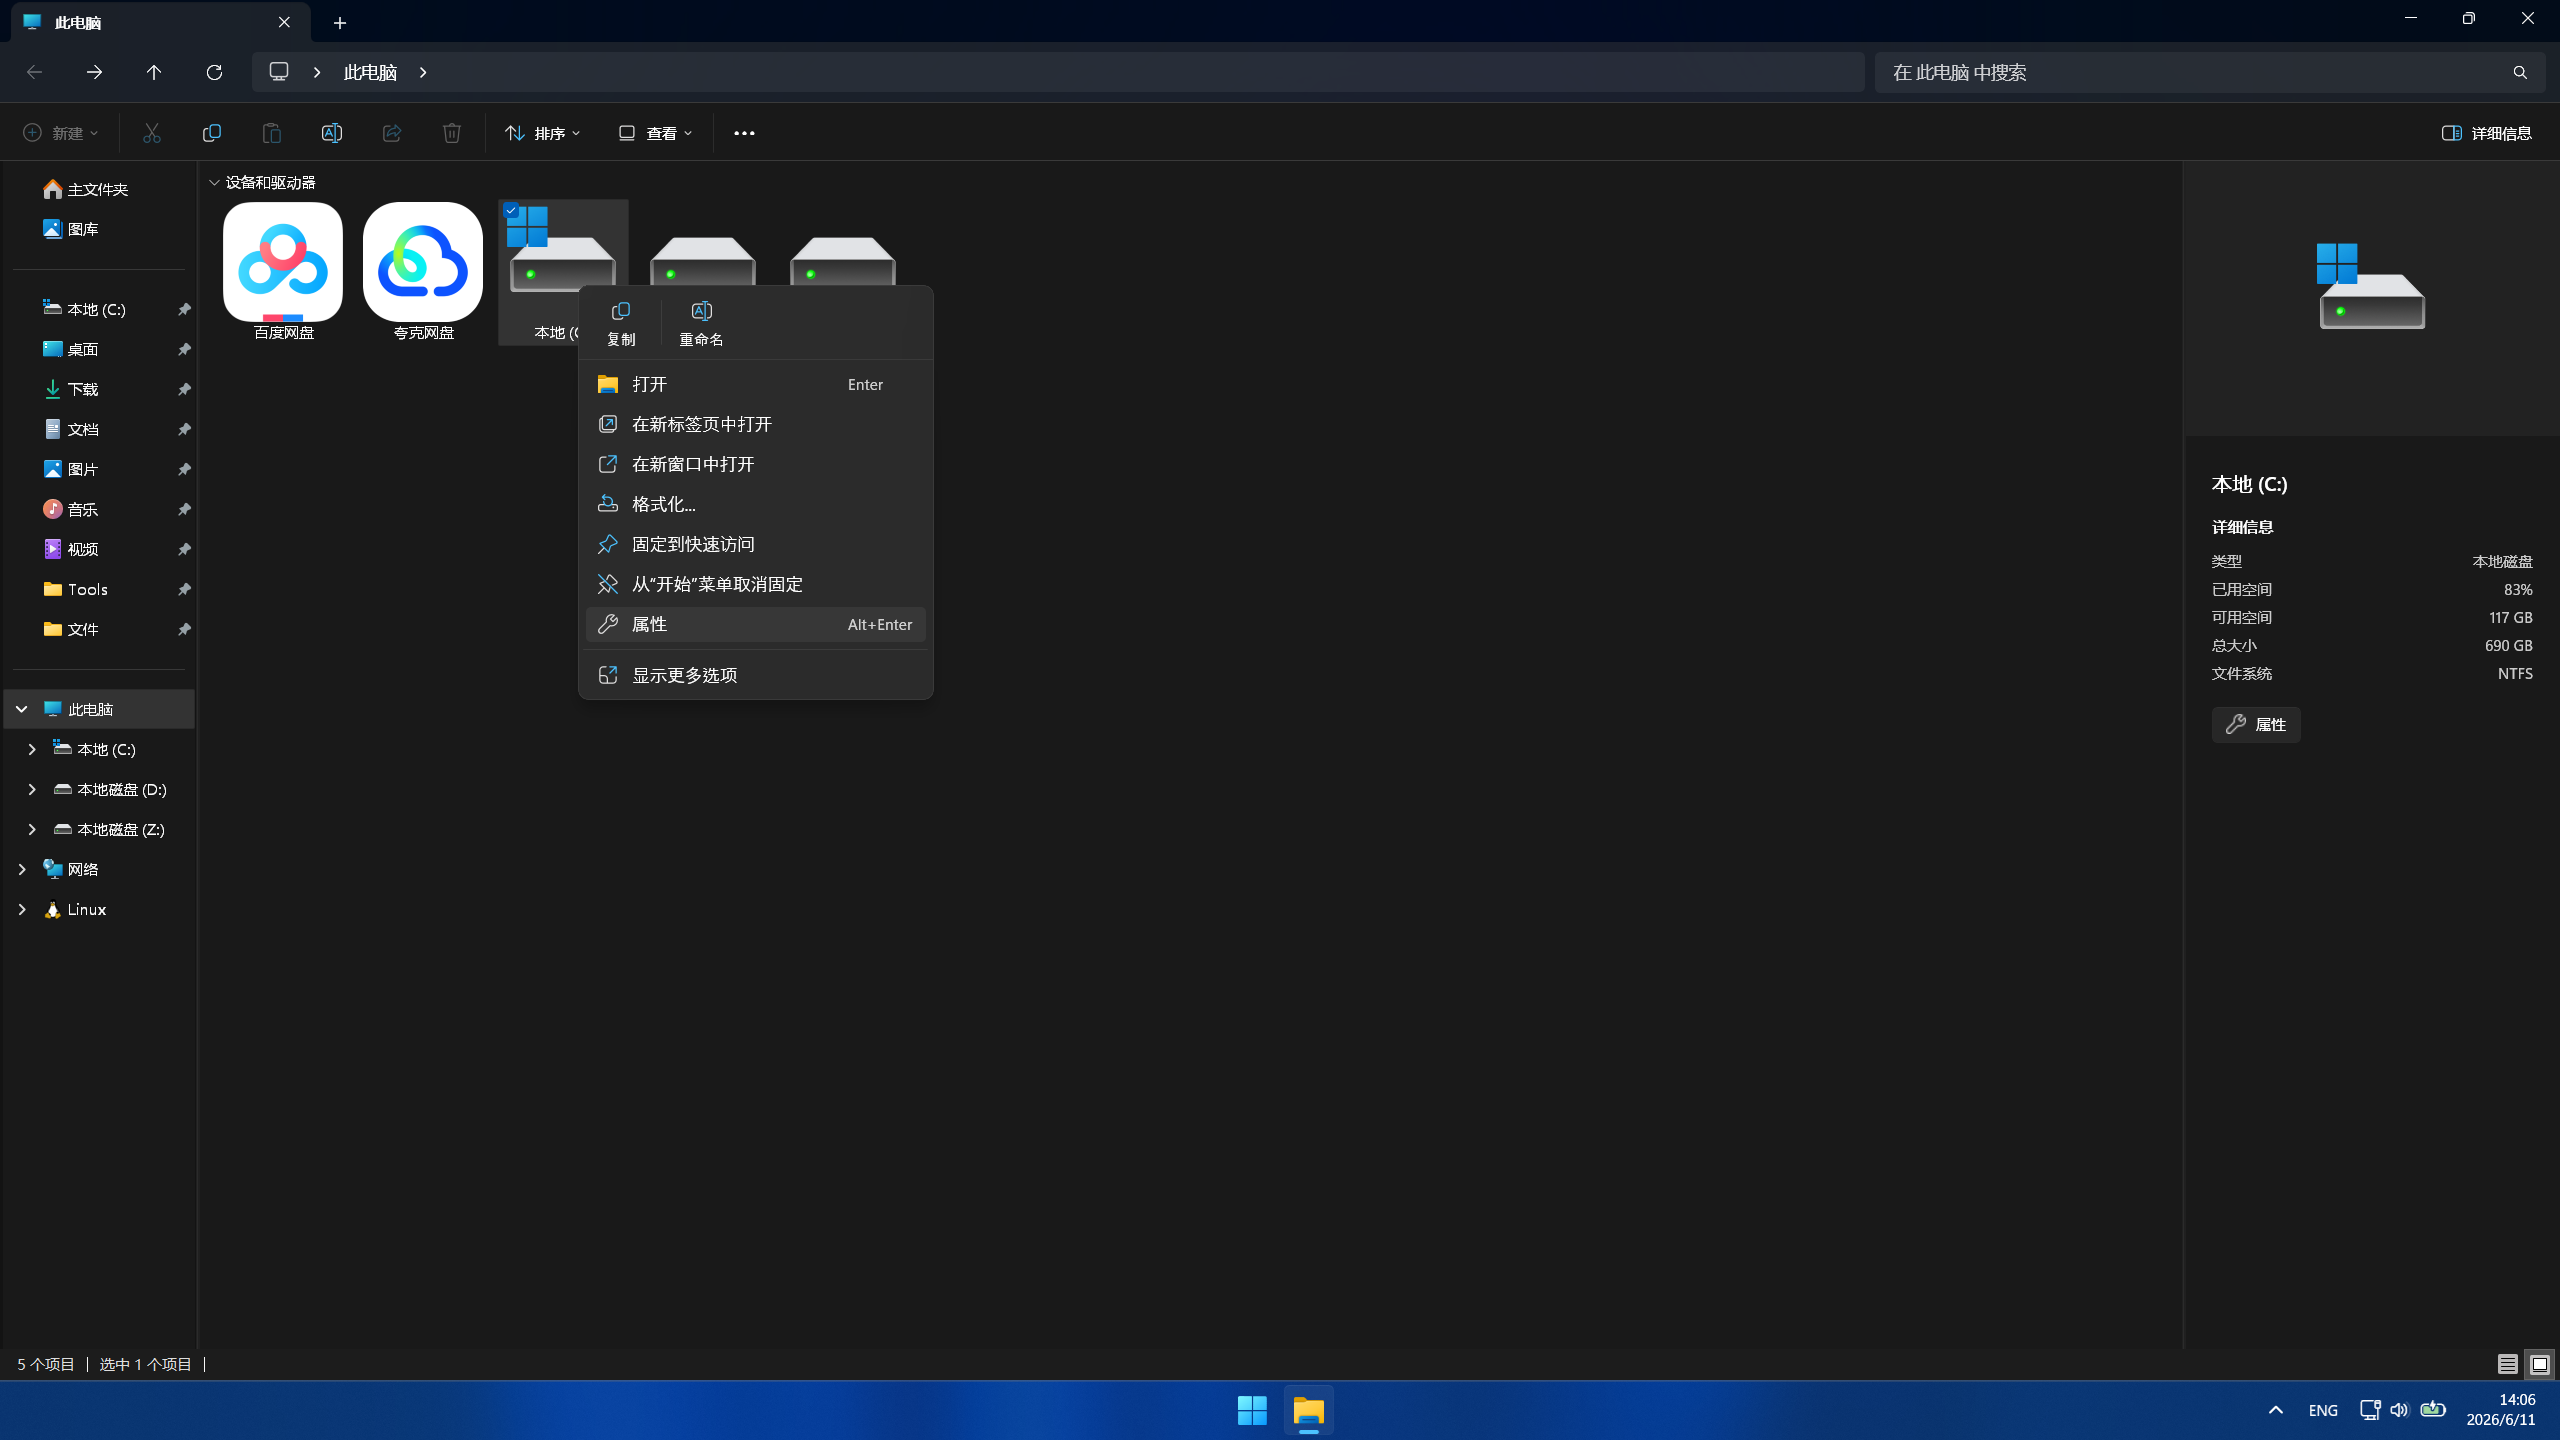
\includegraphics[width=0.5\textwidth]{1.png} 
\end{figure}
\begin{figure}[htbp]
    \centering 
    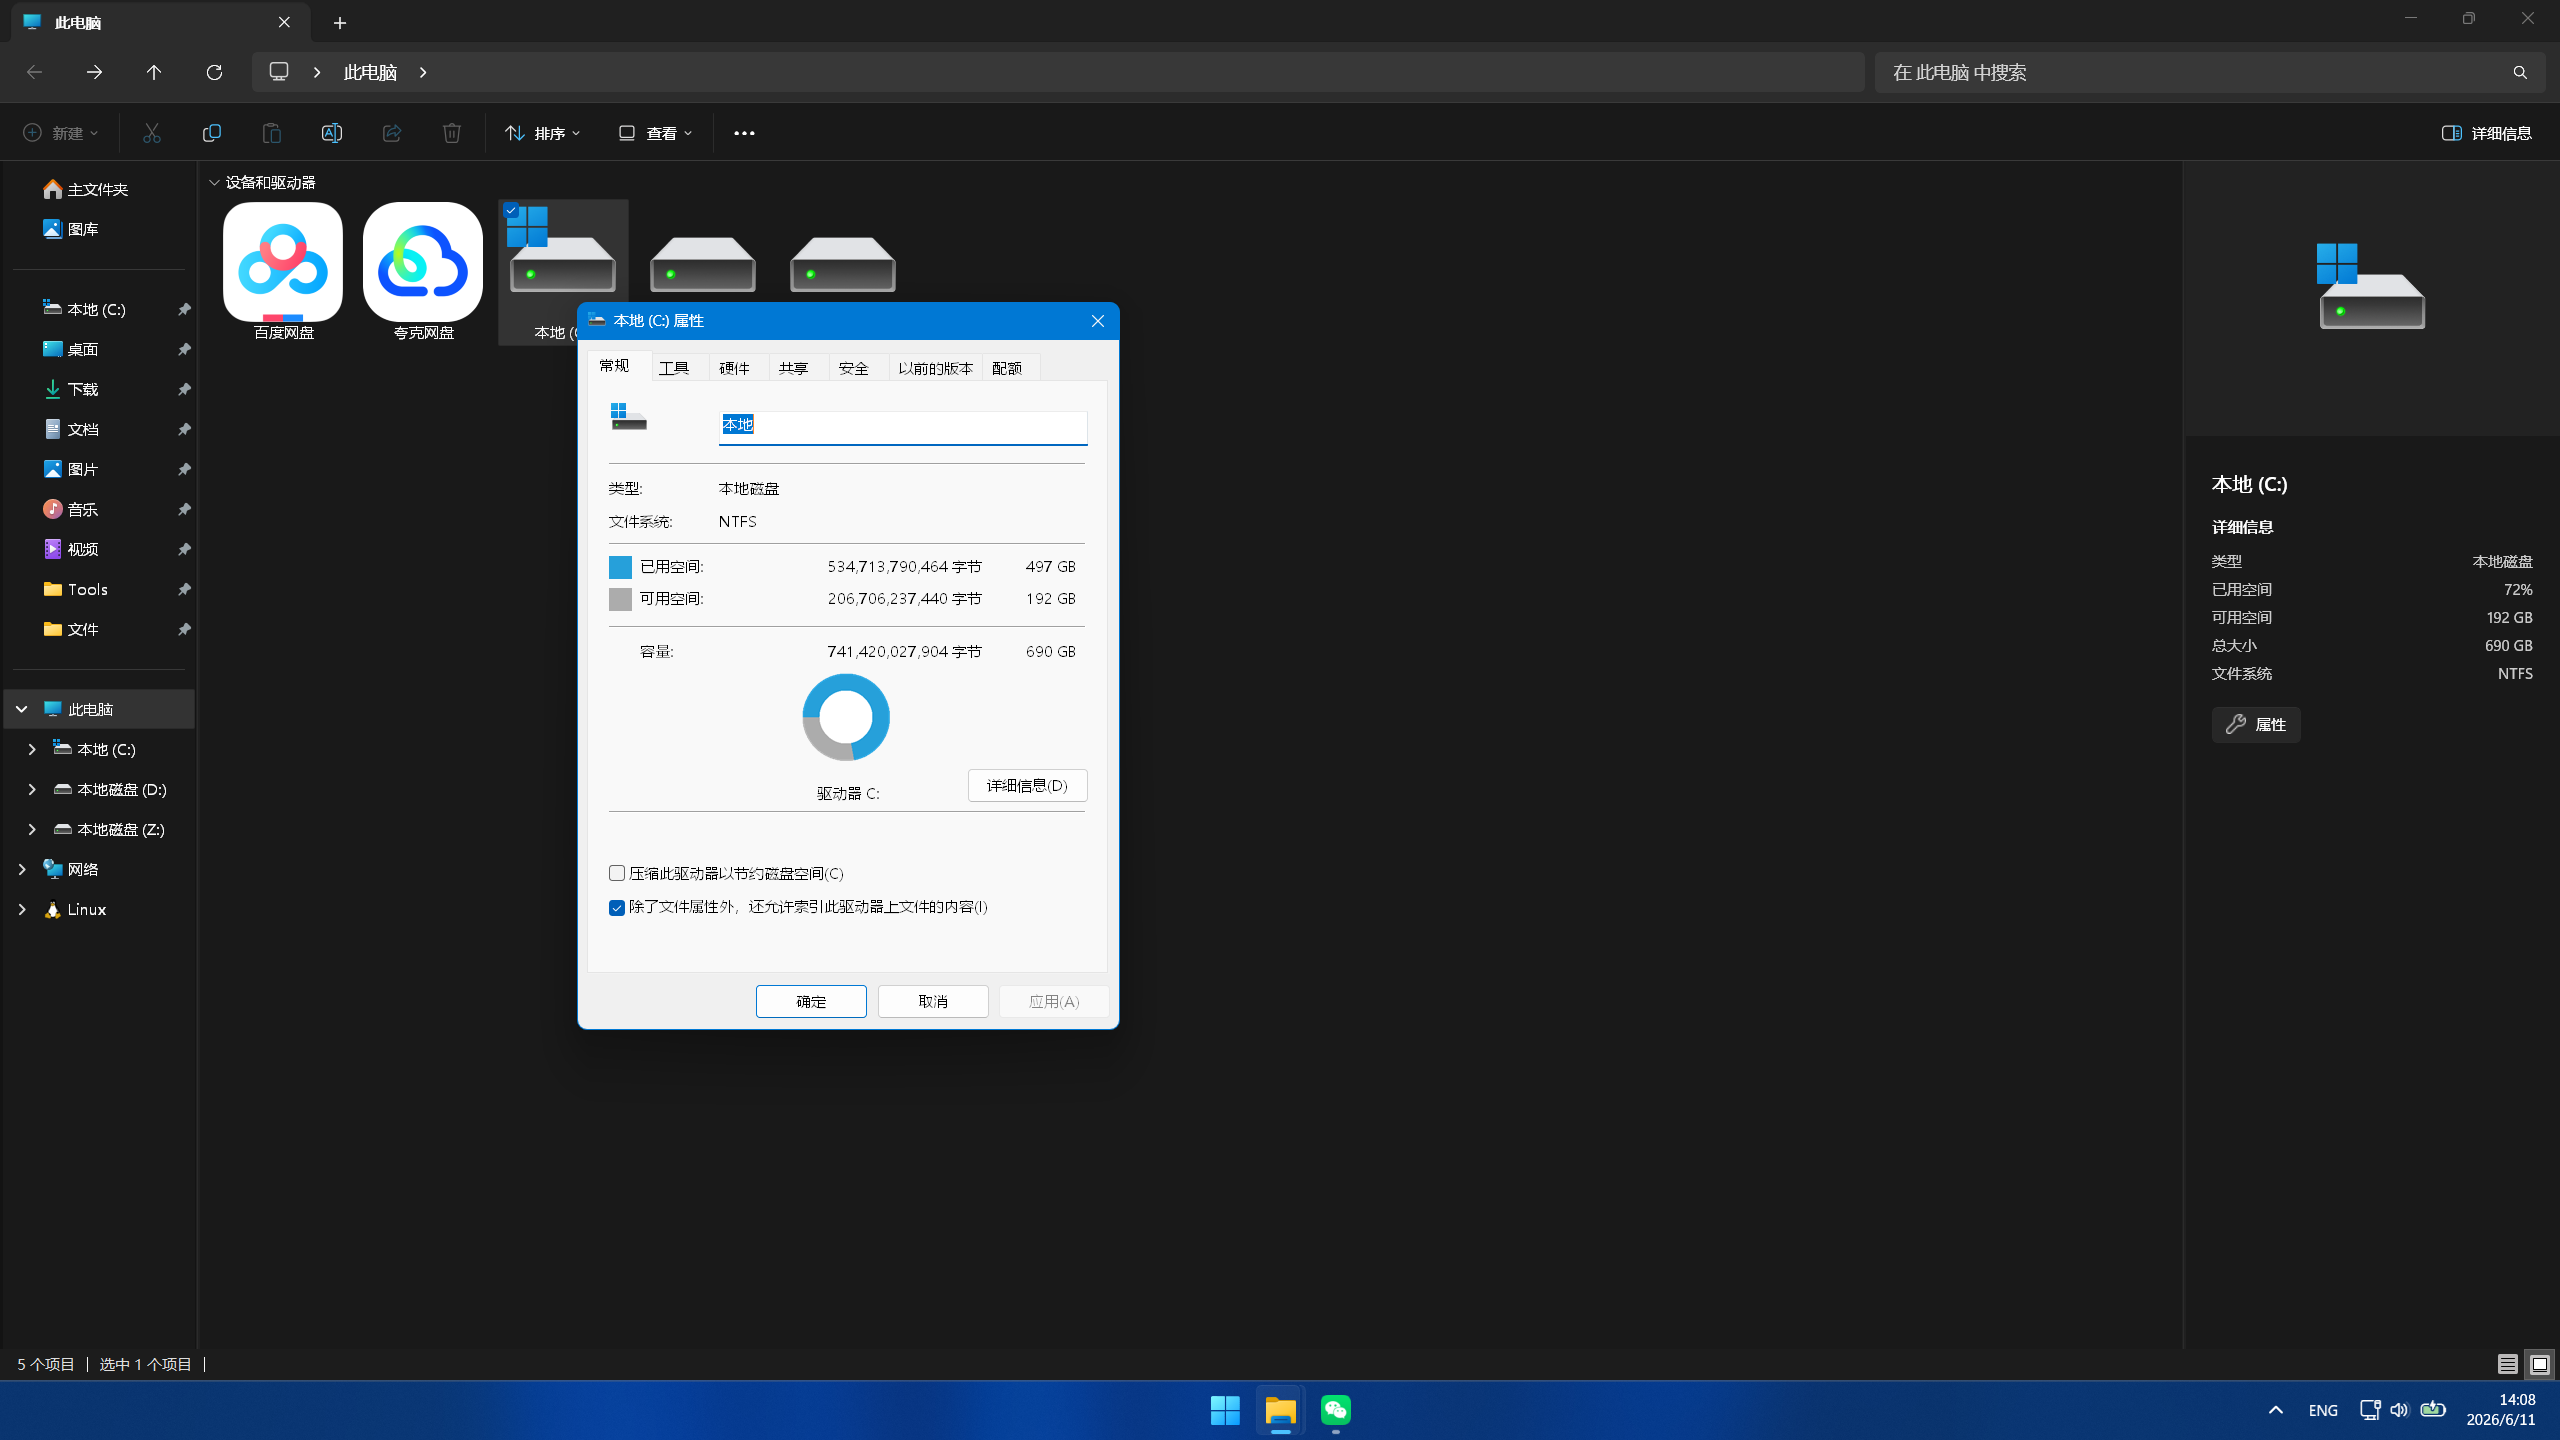
\includegraphics[width=0.5\textwidth]{2.png} 
\end{figure}
如图我的C盘还剩192GB的空间。
\smallbreak
建议至少分配50GB给Ubuntu，如果你有更多的剩余空间，当然越多越好，免得后期不够用。
\newpage
\subsection{腾出空间}
按下 \keys{\cmd + Q} 或 \keys{\cmd + S} 打开Windows的搜索页面。

搜索”磁盘管理“。

打开”创建并格式化硬盘分区“。
\begin{figure}[H]
    \centering 
    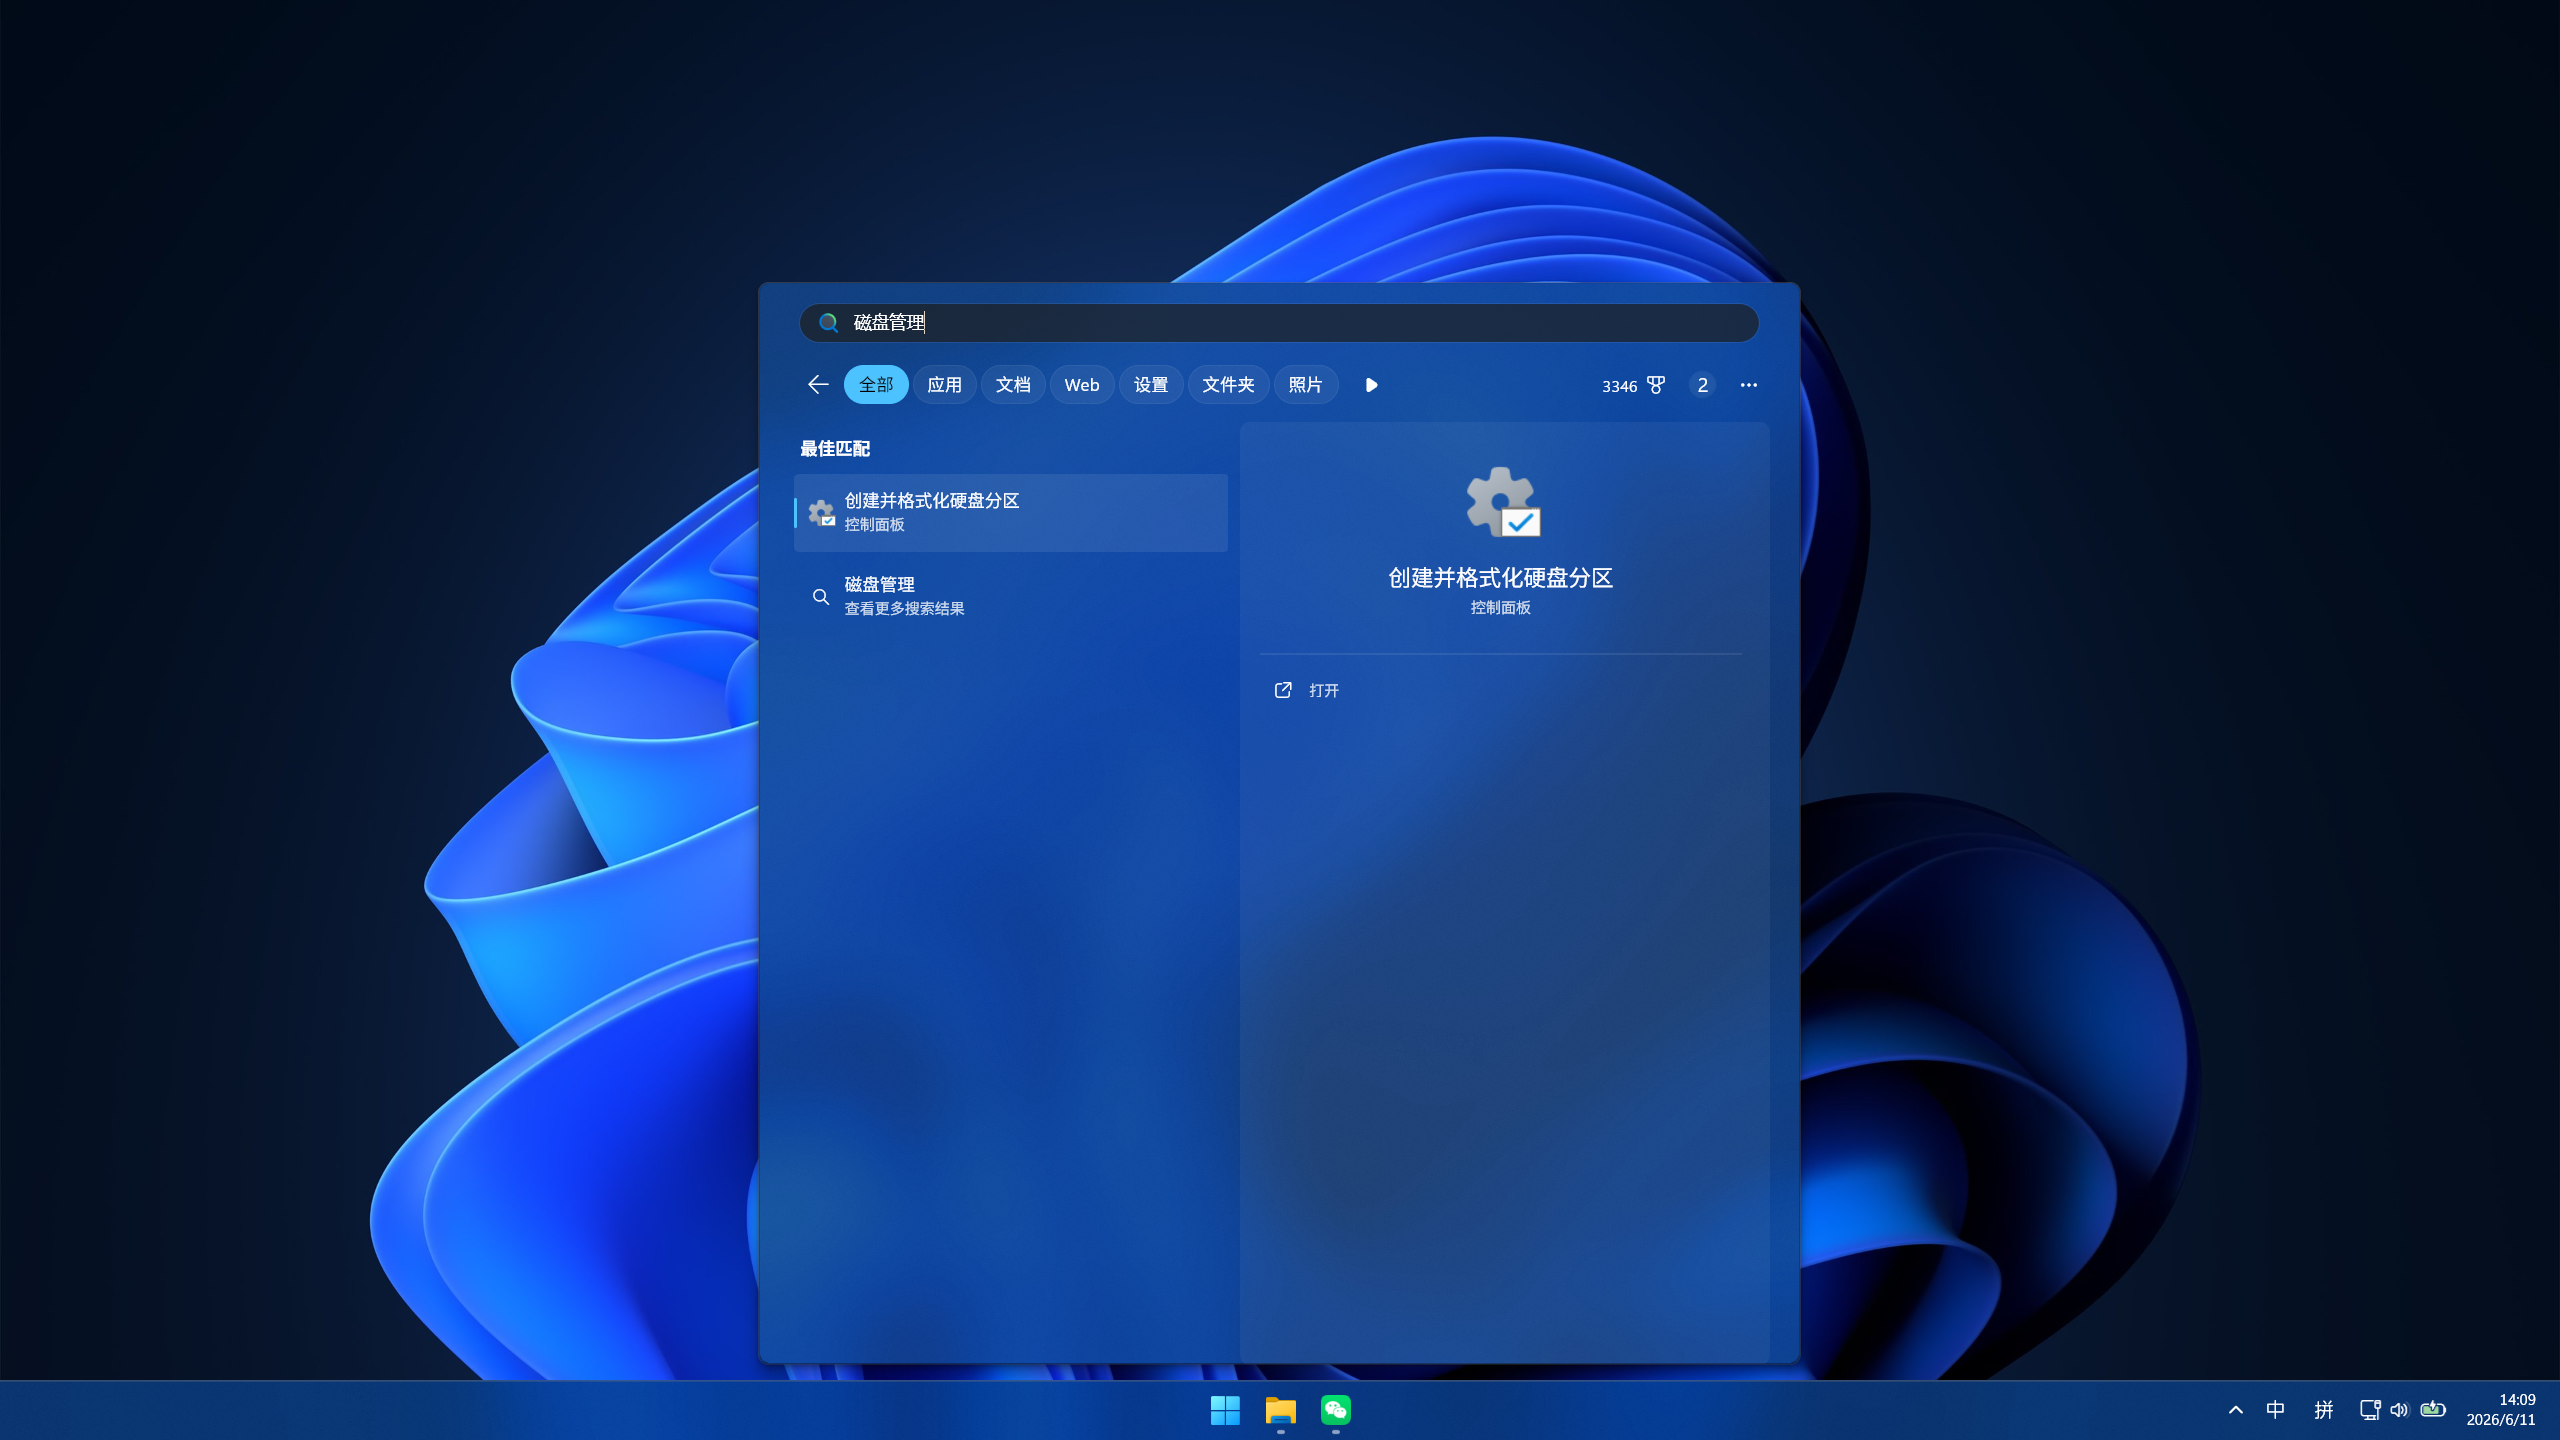
\includegraphics[width=0.7\textwidth]{4.png} 
\end{figure}
\begin{figure}[H]
    \centering 
    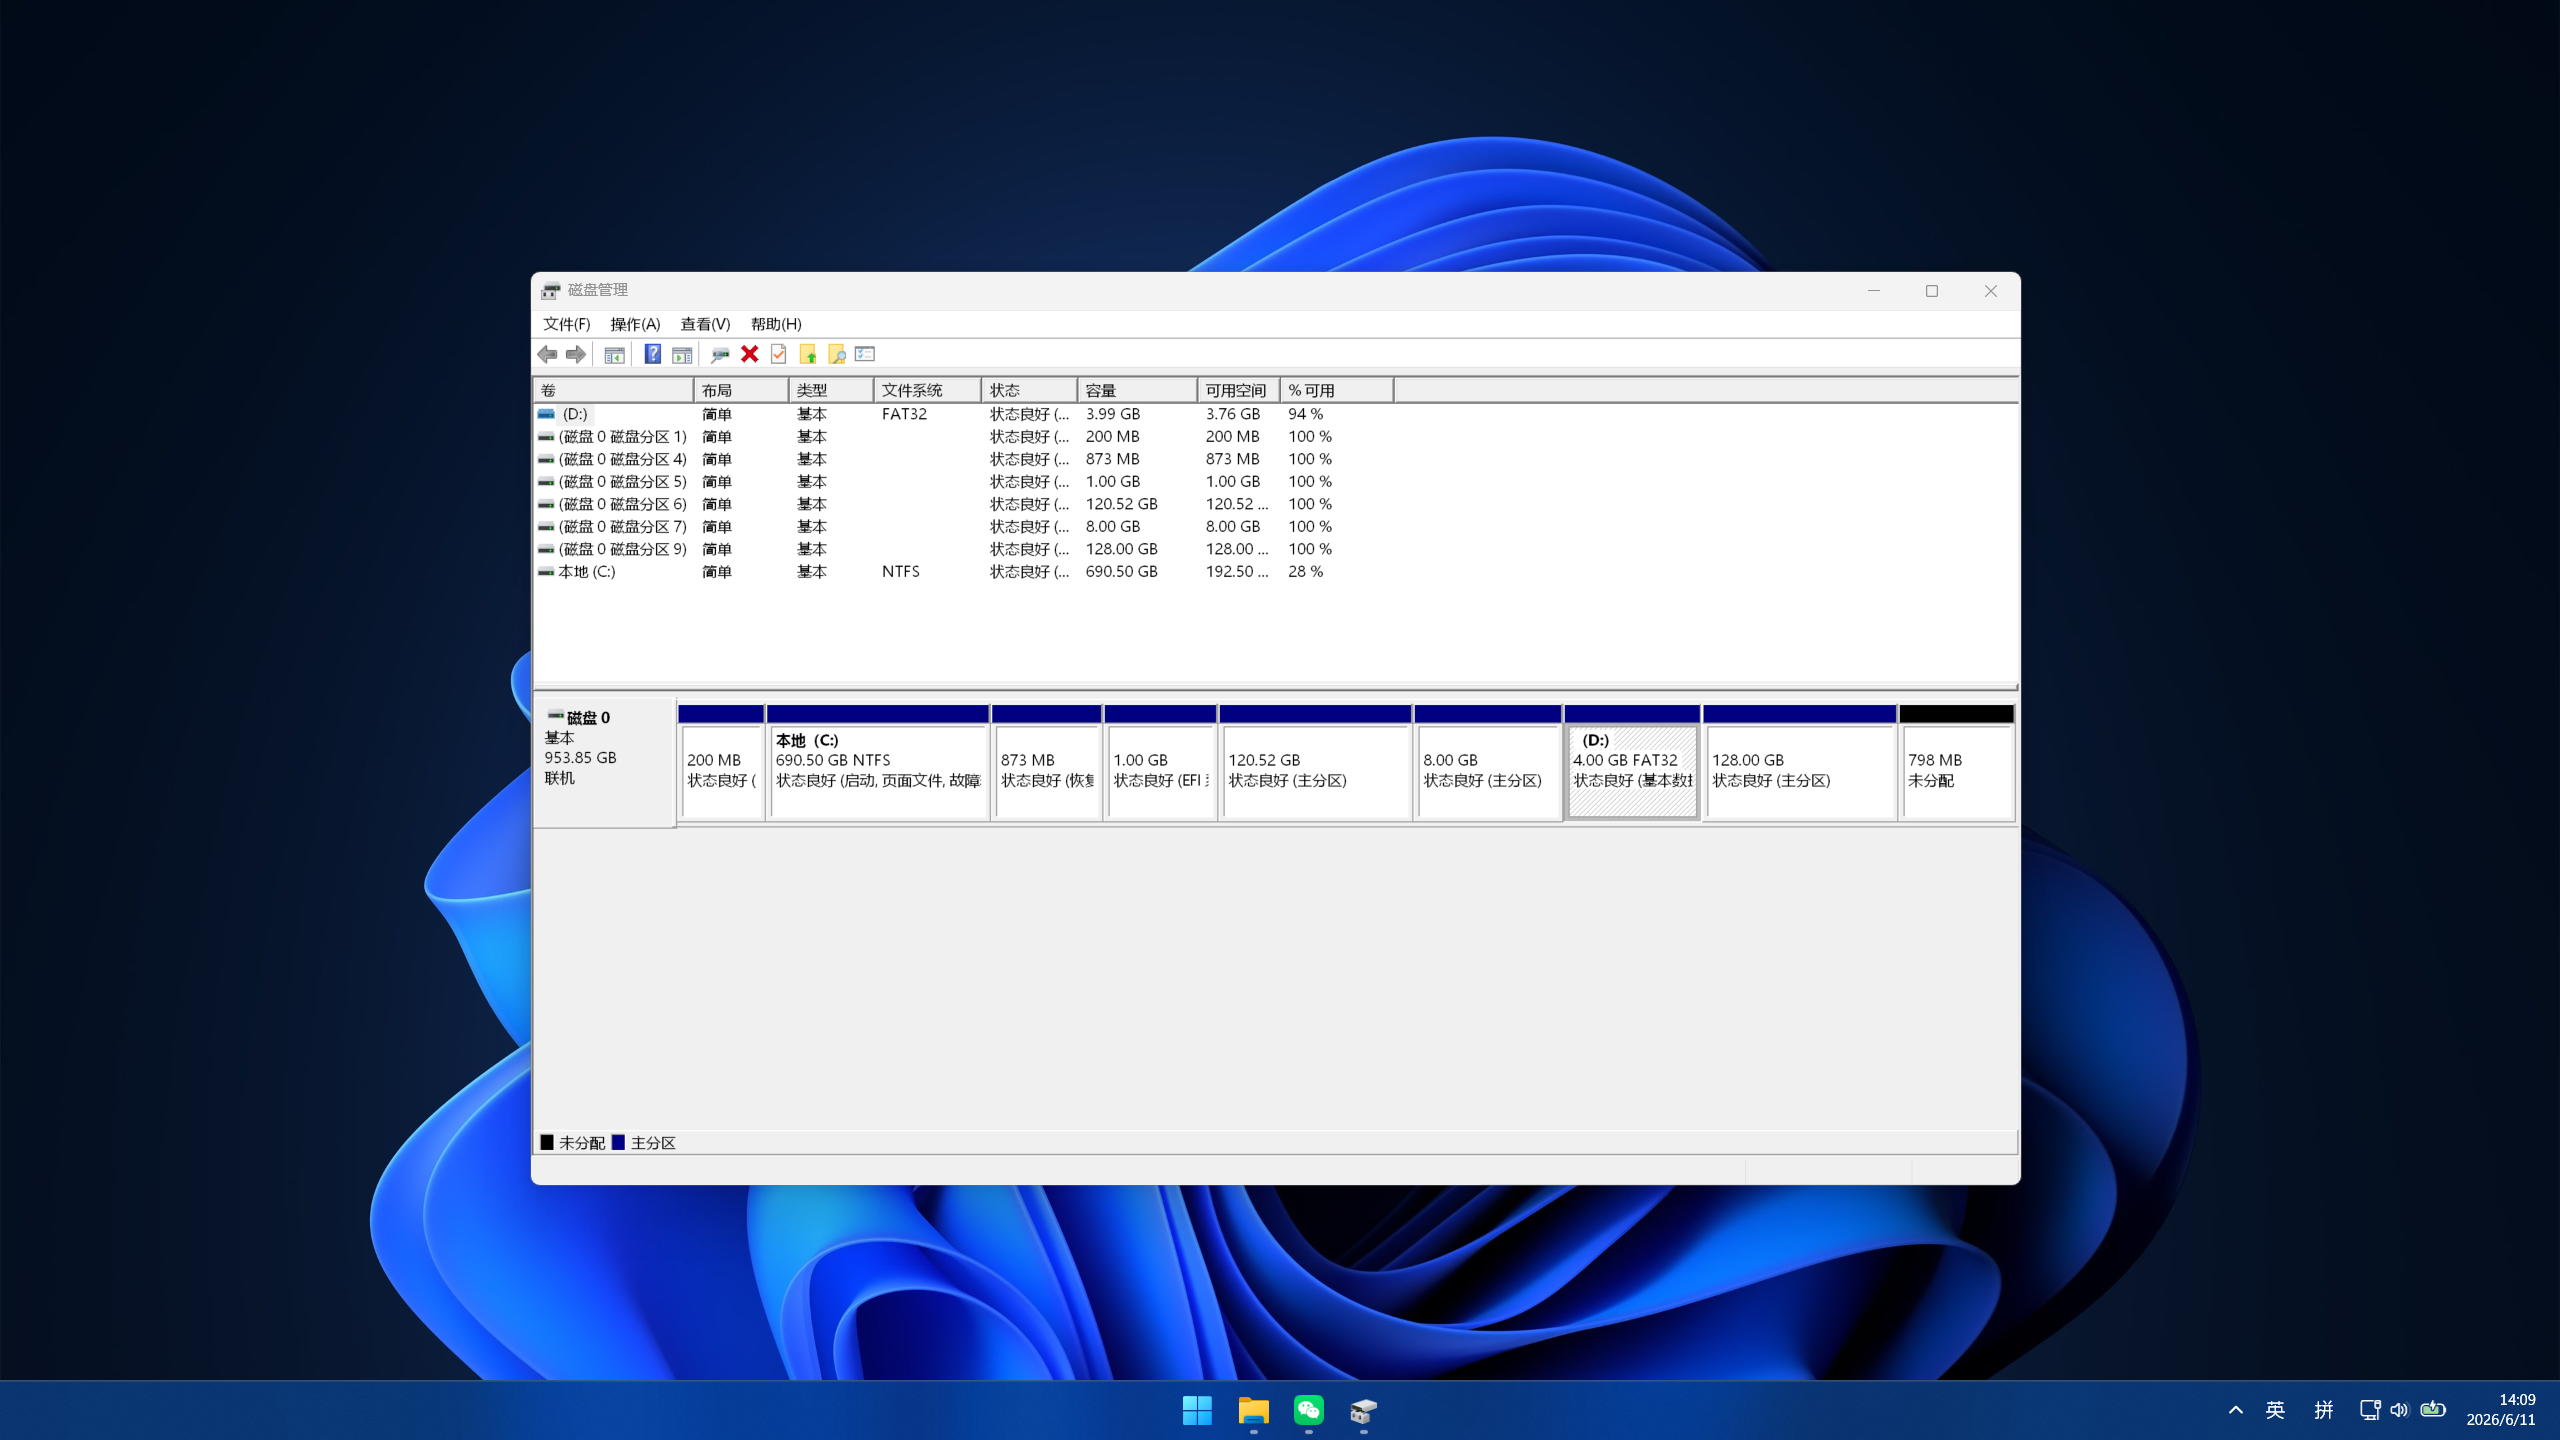
\includegraphics[width=0.7\textwidth]{5.png} 
\end{figure}
如下图，右击要给Ubuntu分配空间的磁盘（如C盘），选择”压缩卷“。
\begin{figure}[H]
    \centering 
    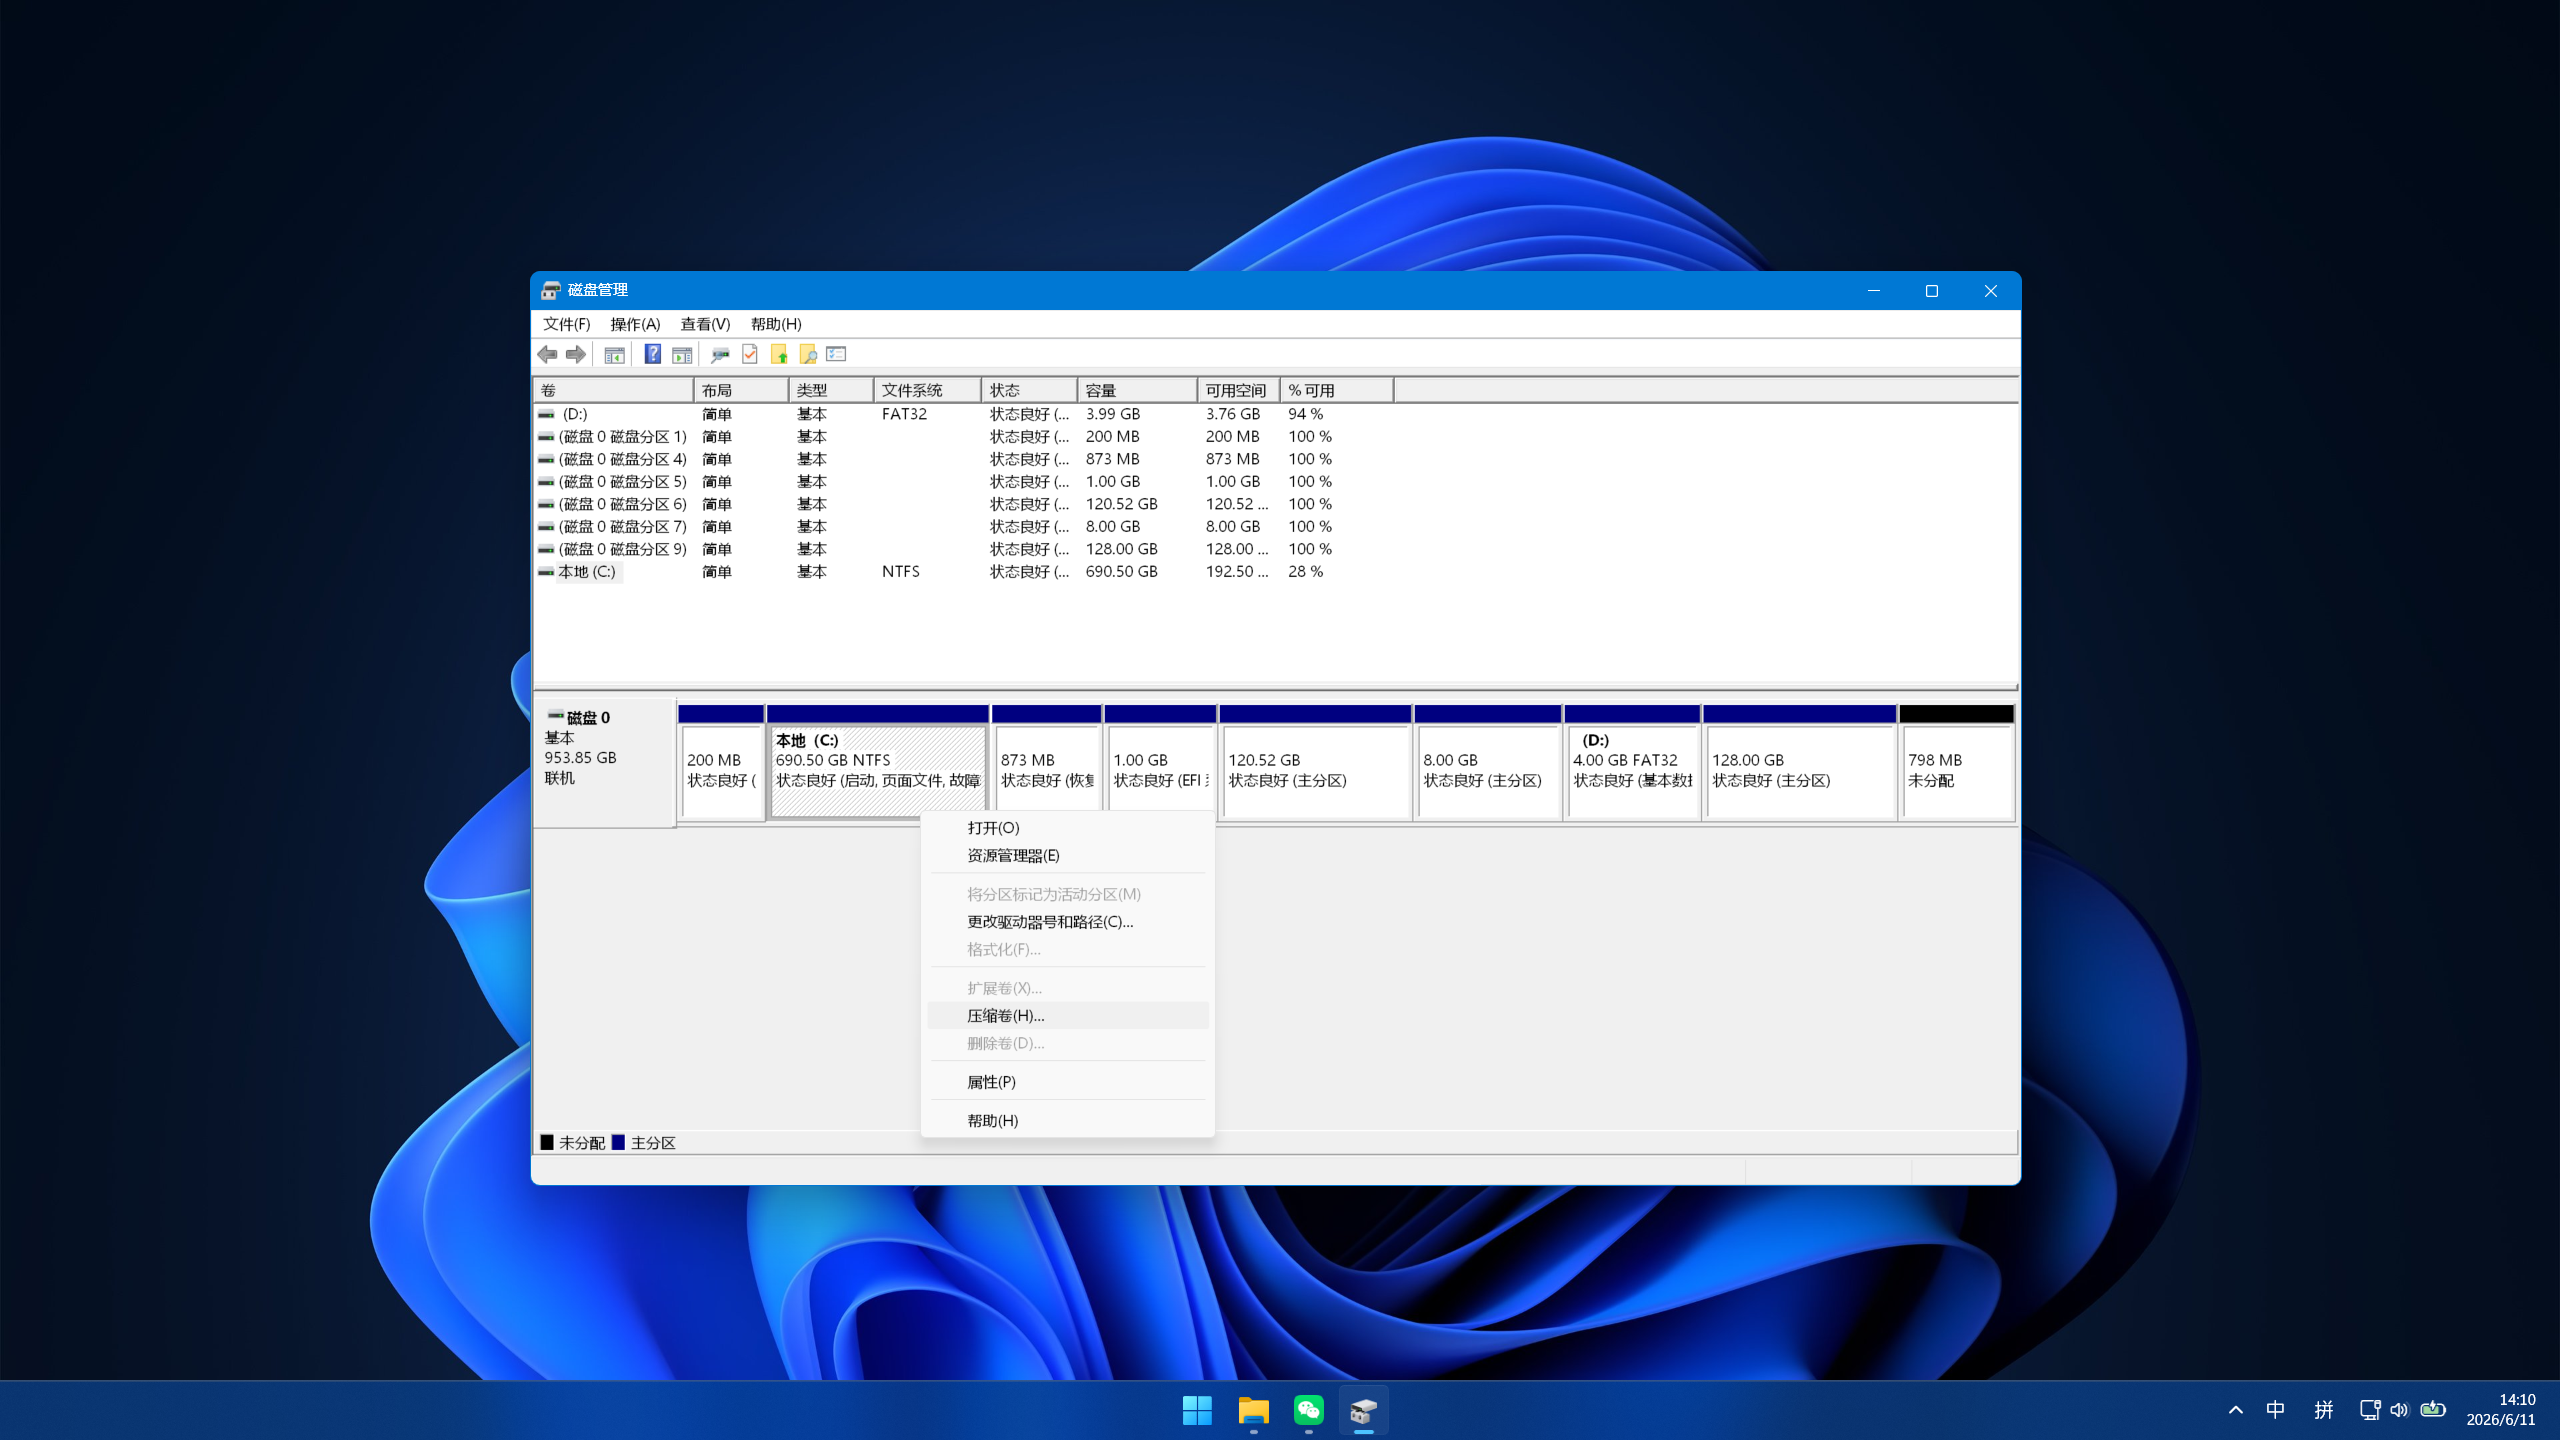
\includegraphics[width=0.7\textwidth]{6.png} 
\end{figure}
如下图，在弹窗里输入压缩空间量。(我的C盘明明还有192GB的剩余空间，但是截图里却显示可用压缩空间大小只有47461MB，这是因为盘里有不可移动的文件挡在了中间，如果要压缩超过这个大小的空间，就需要用到例如”傲梅分区助手“等第三方工具了。)
\begin{figure}[H]
    \centering 
    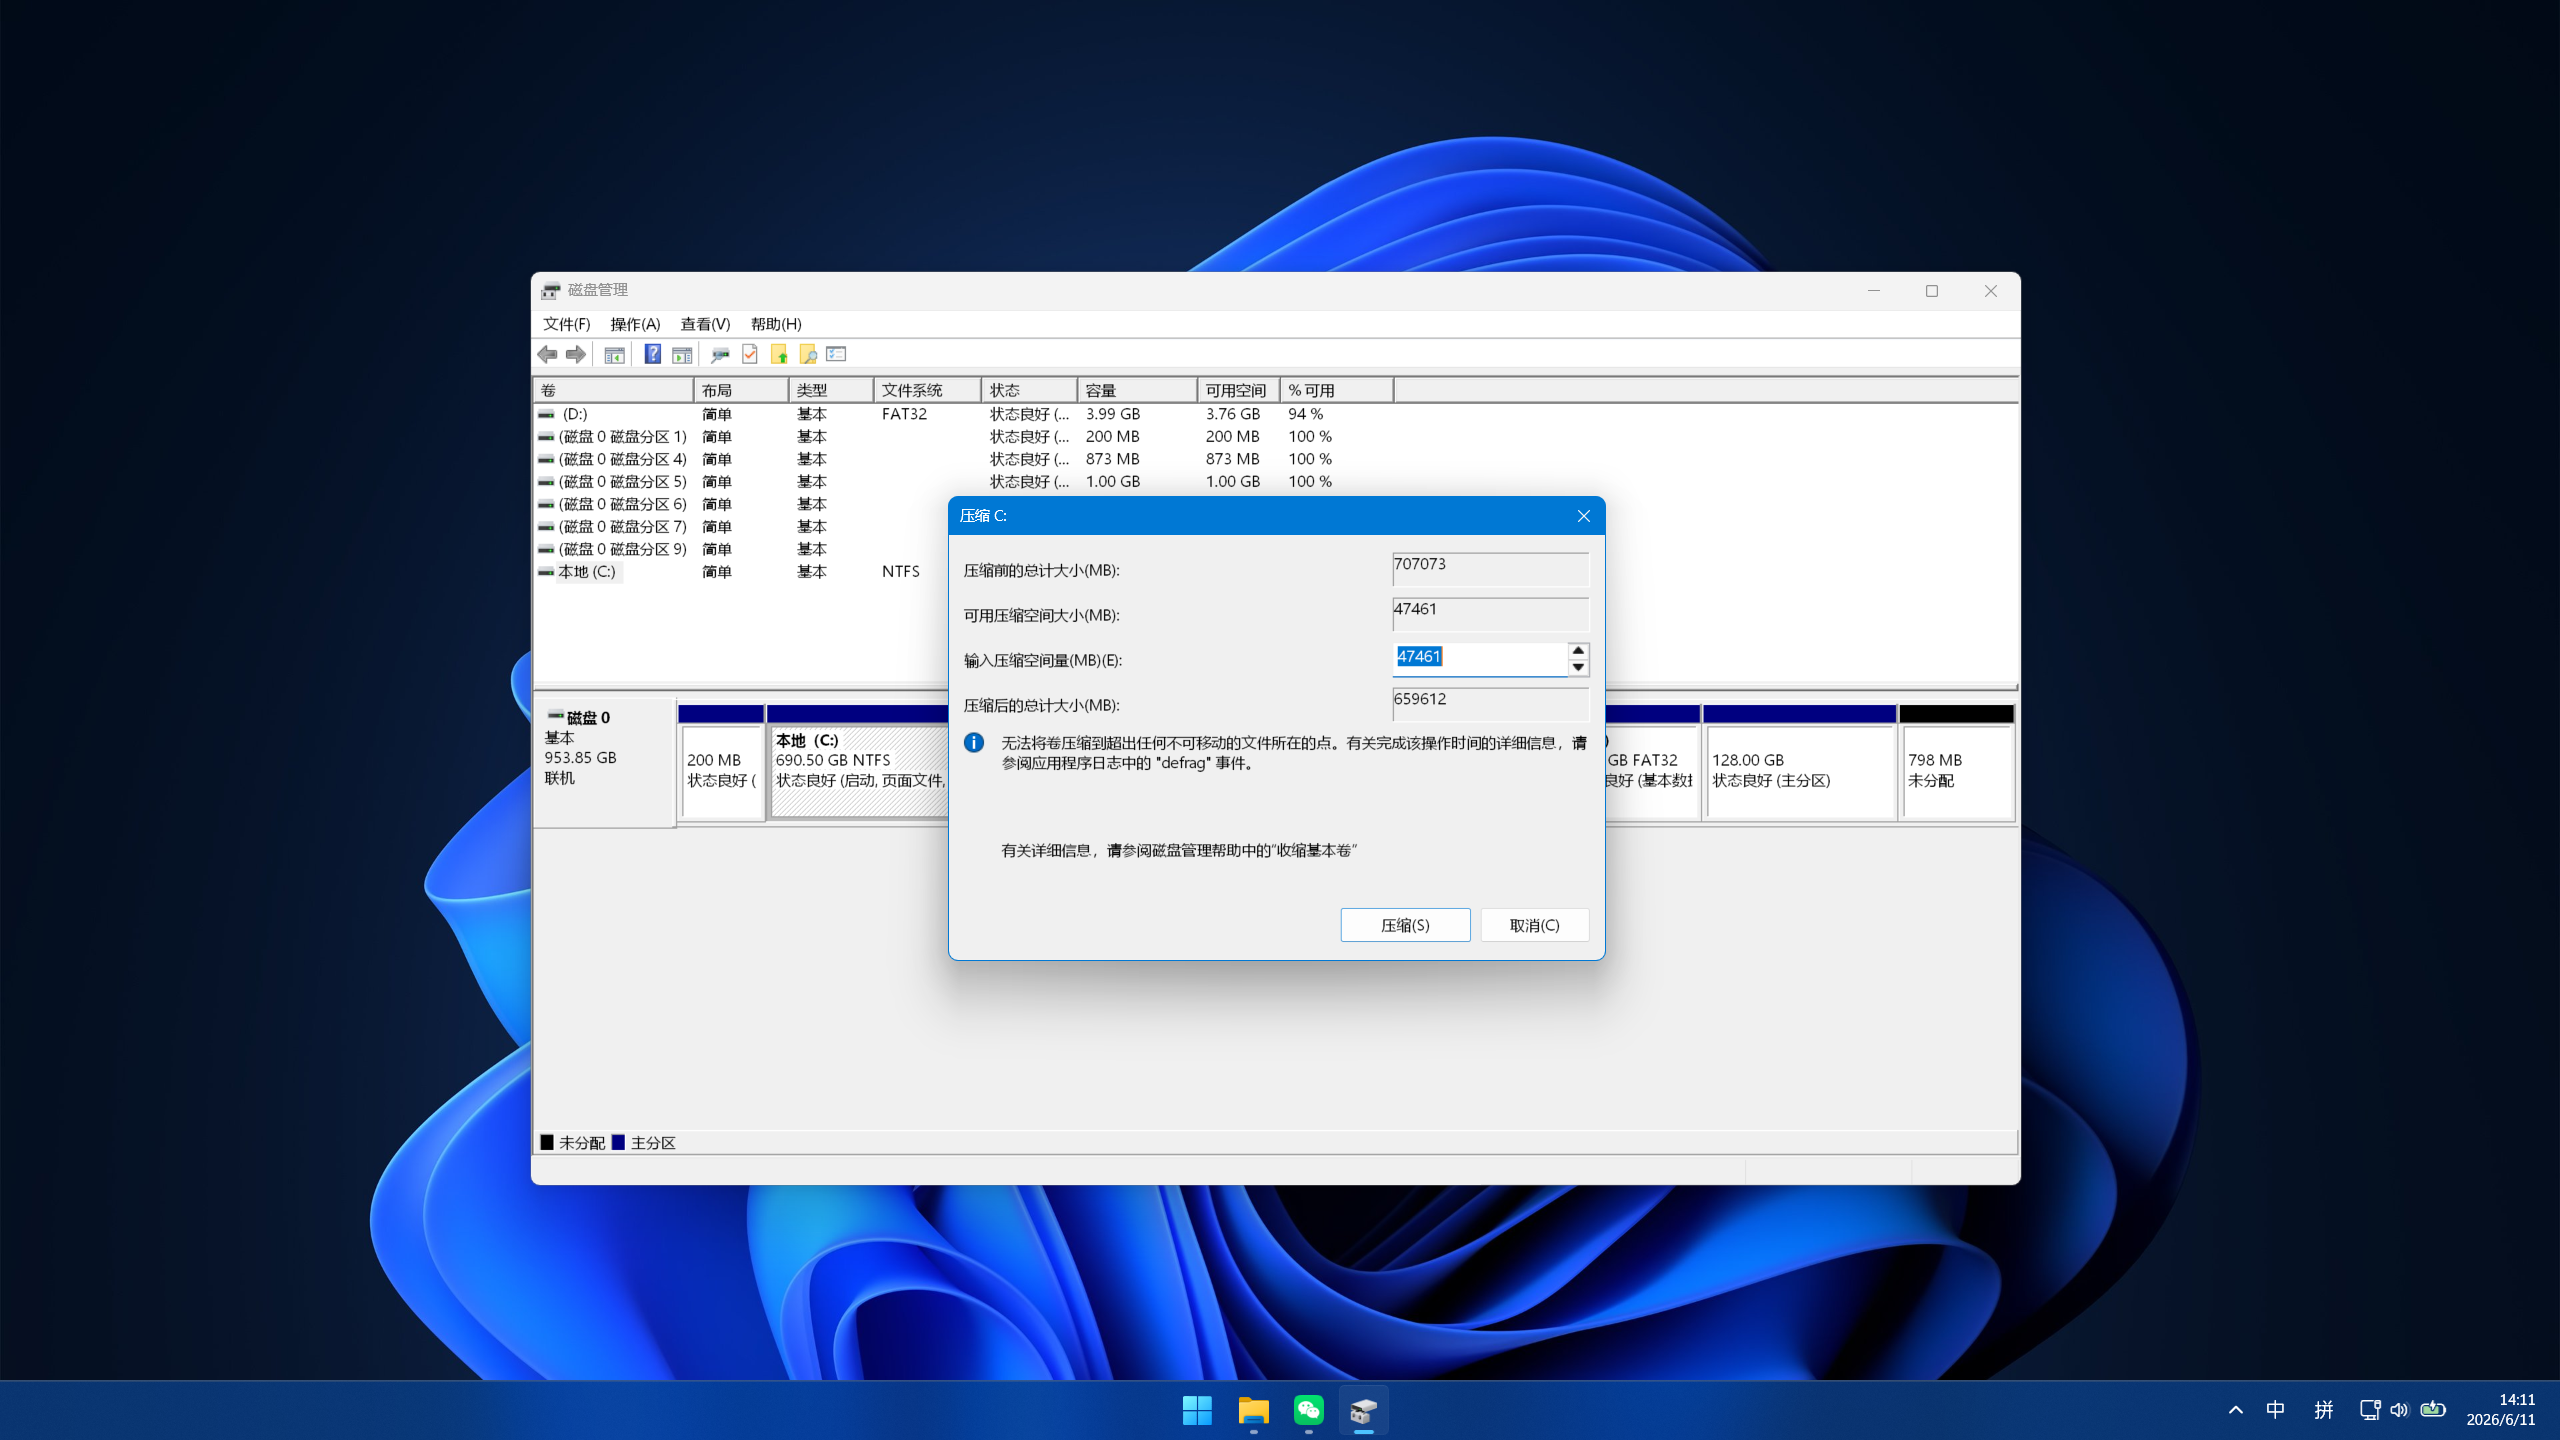
\includegraphics[width=0.7\textwidth]{7.png} 
\end{figure}
选择好要压缩的空间大小后，点击”压缩“，就会在磁盘管理里看到一个黑的未分配的空间了。如下图，我选择了压缩47461MB，所以我有了46.35GB的未分配空间。这个未分配的空间就是给Ubuntu安装用的。
\begin{figure}[H]
    \centering 
    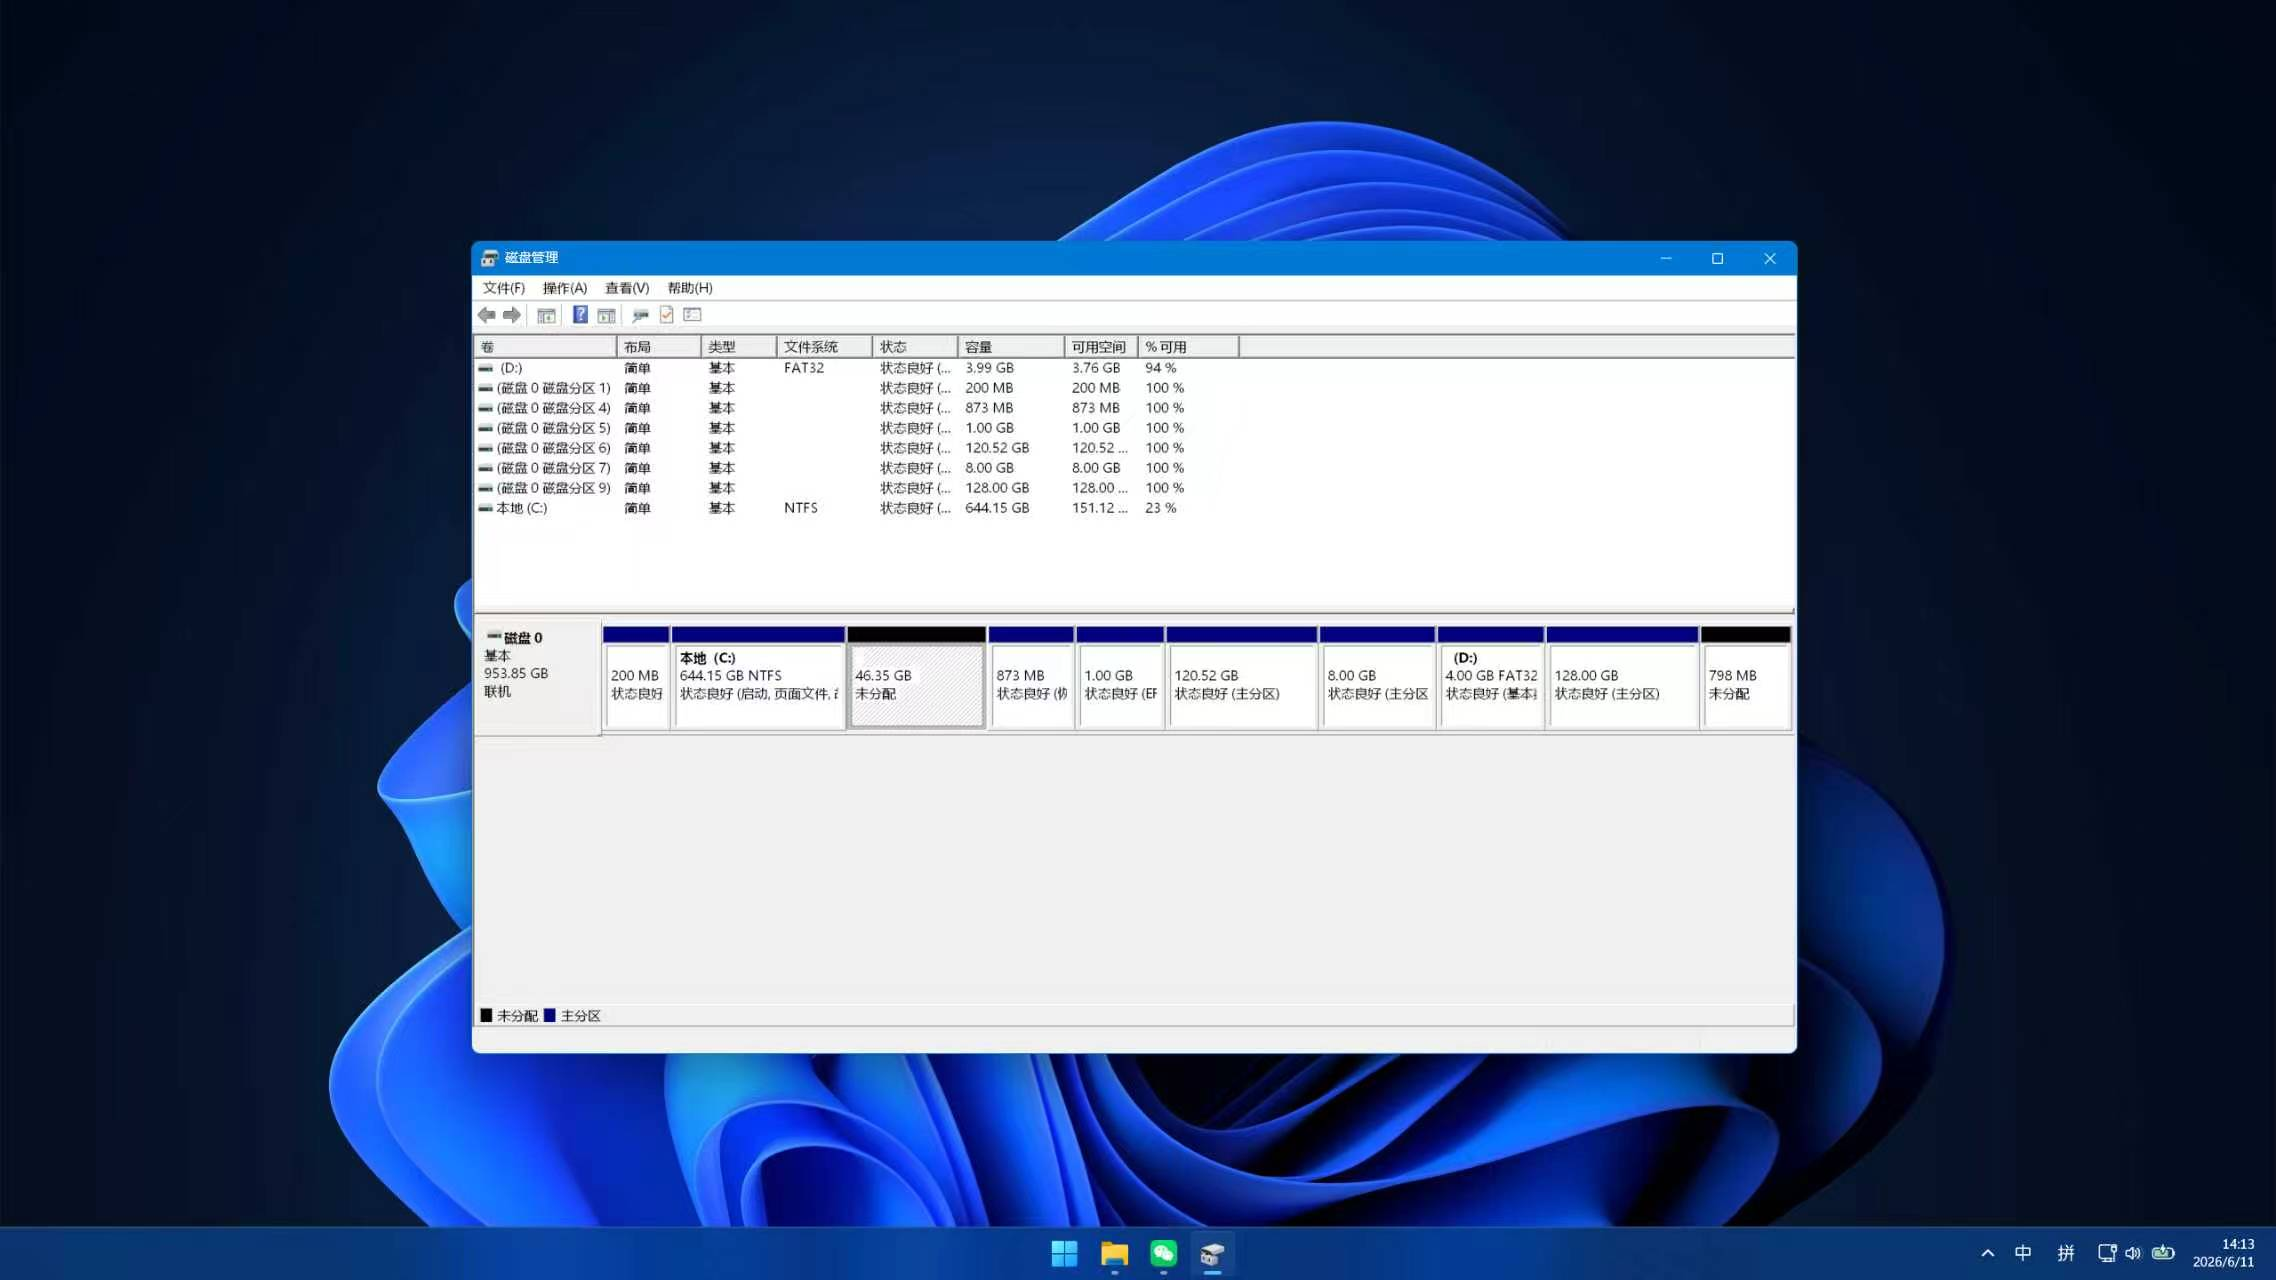
\includegraphics[width=0.7\textwidth]{8.jpg} 
\end{figure}
\newpage

\section{修改电脑设置}
\subsection{关闭windows的休眠功能}
按下 \keys{\cmd + Q} 或 \keys{\cmd + S} 打开Windows的搜索页面，搜索\textbf{cmd}。
\smallbreak
不要直接点"打开"，而是点击"以管理员身份运行"。
\begin{figure}[H]
    \centering 
    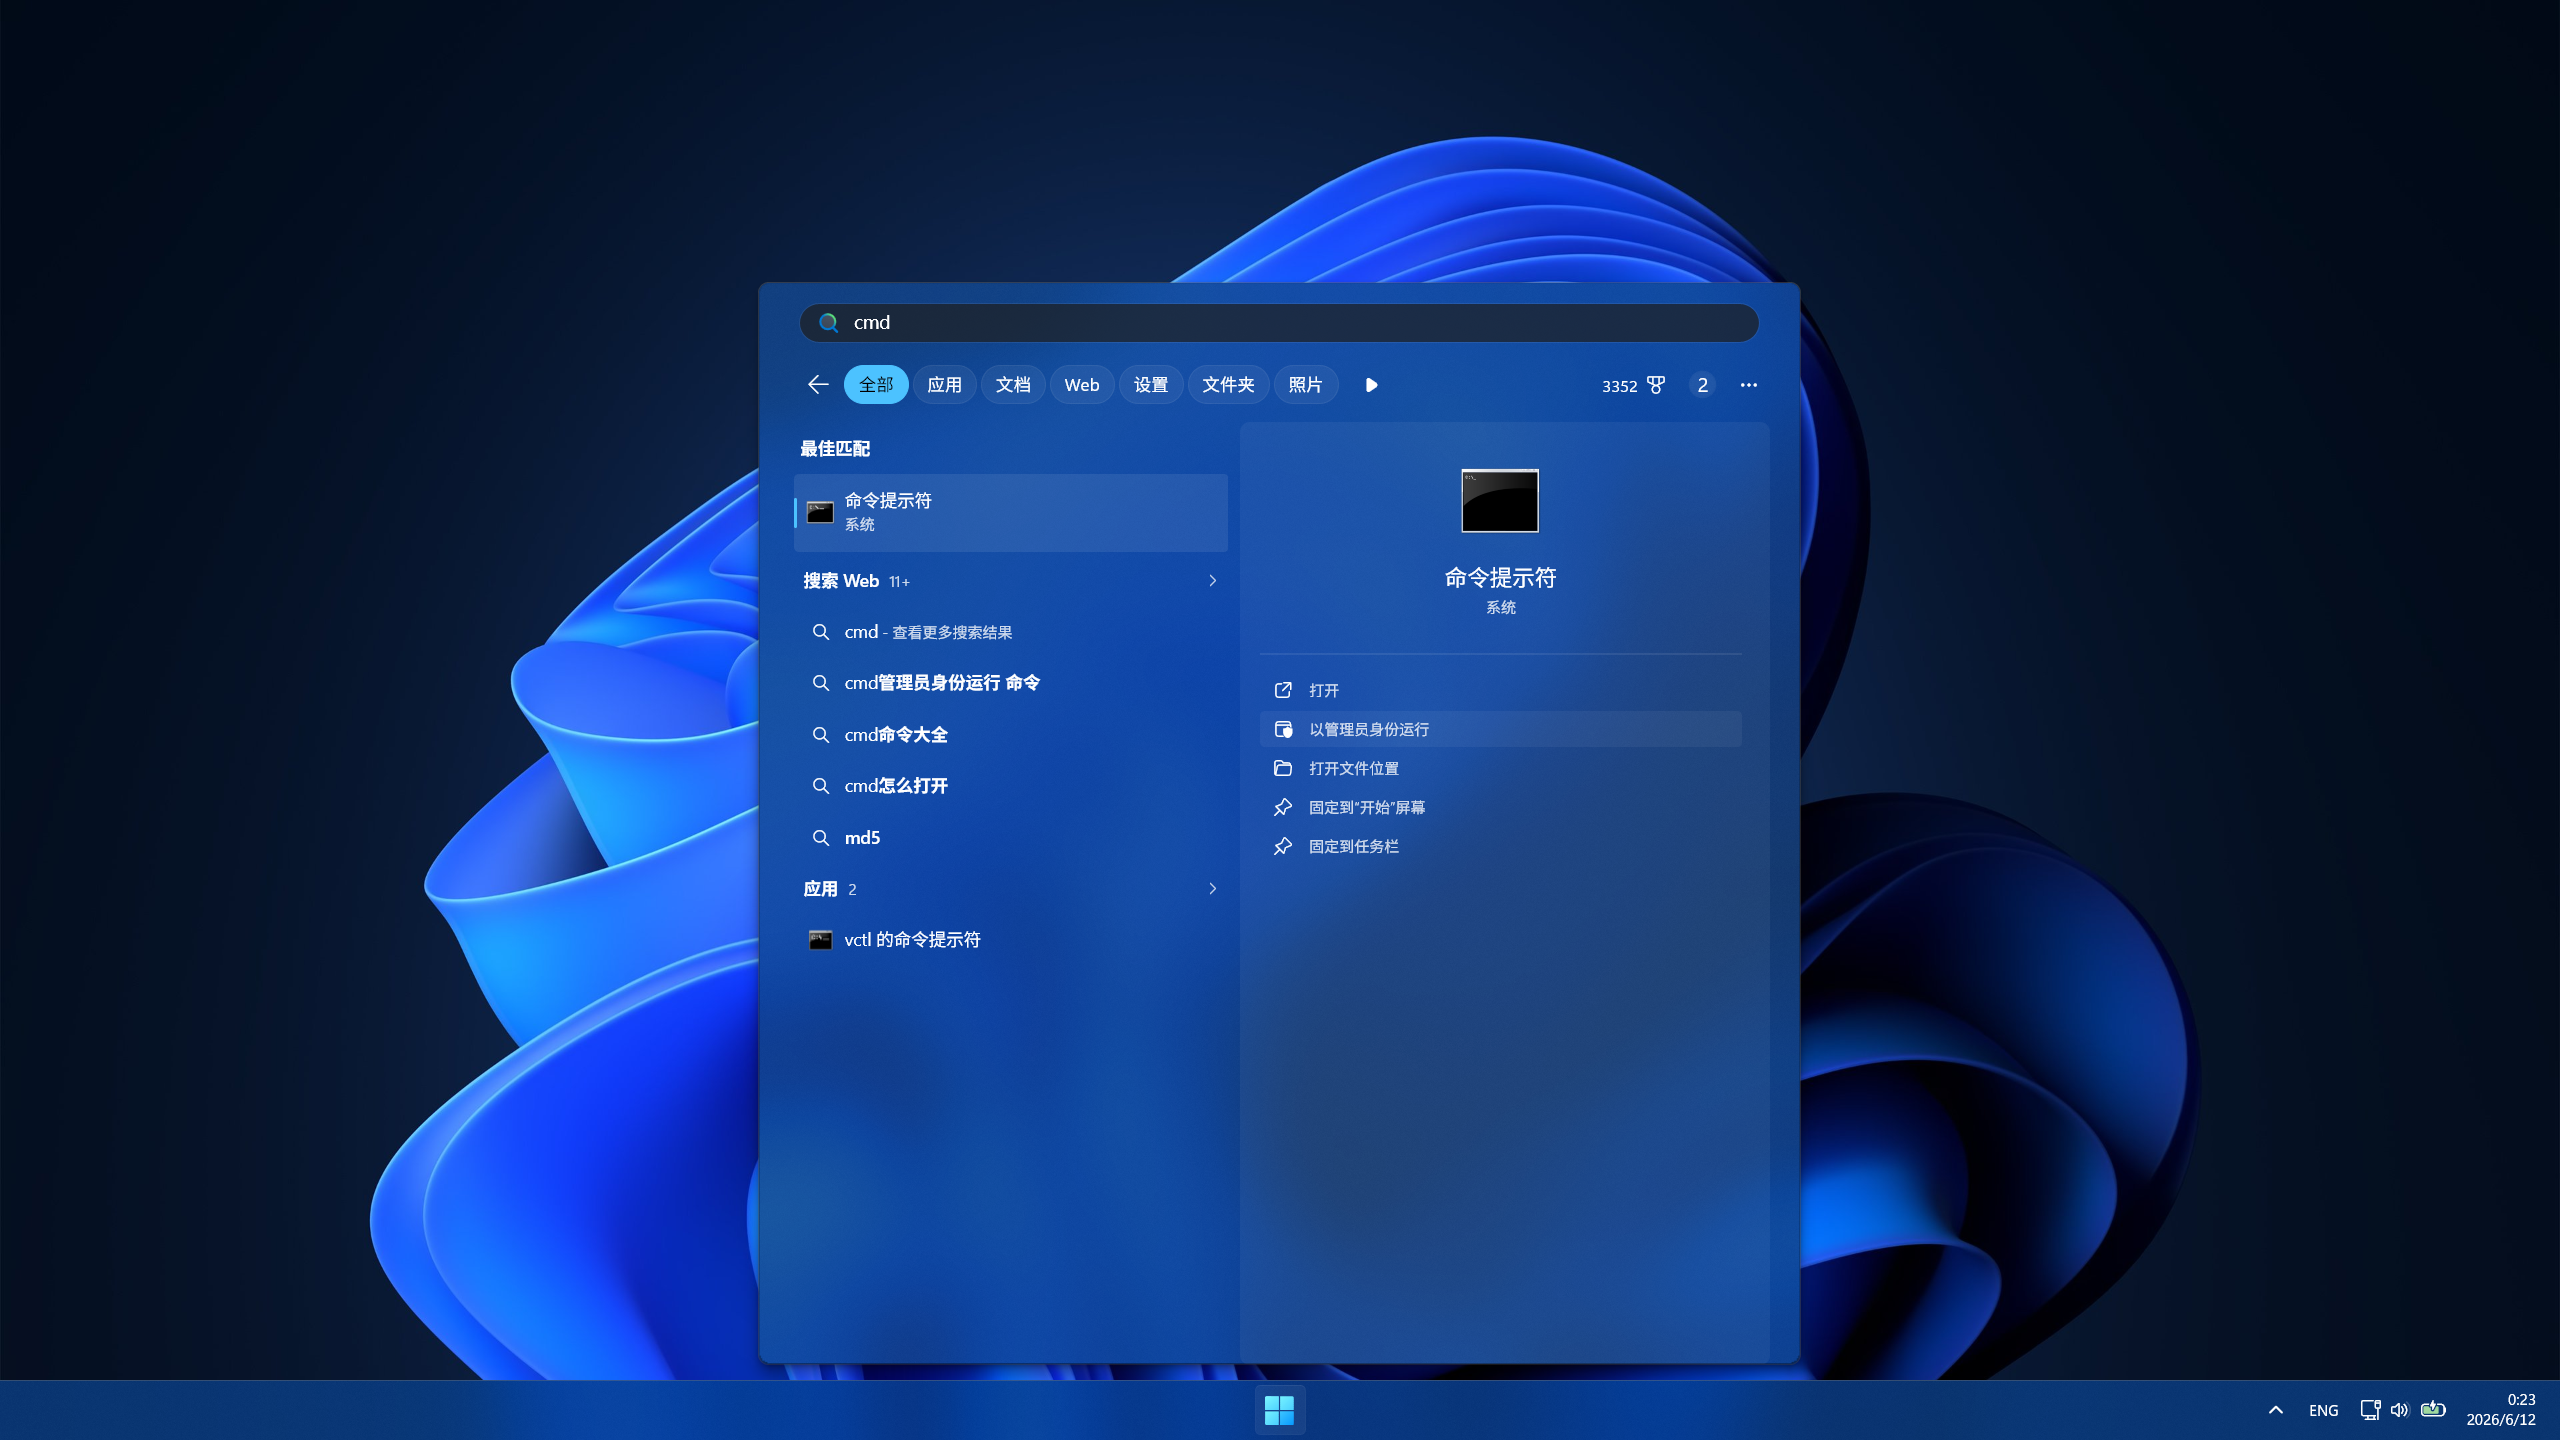
\includegraphics[width=0.8\textwidth]{9.png} 
\end{figure}
输入命令 \texttt{powercfg /h off} 来关闭休眠功能。
\begin{figure}[H]
    \centering 
    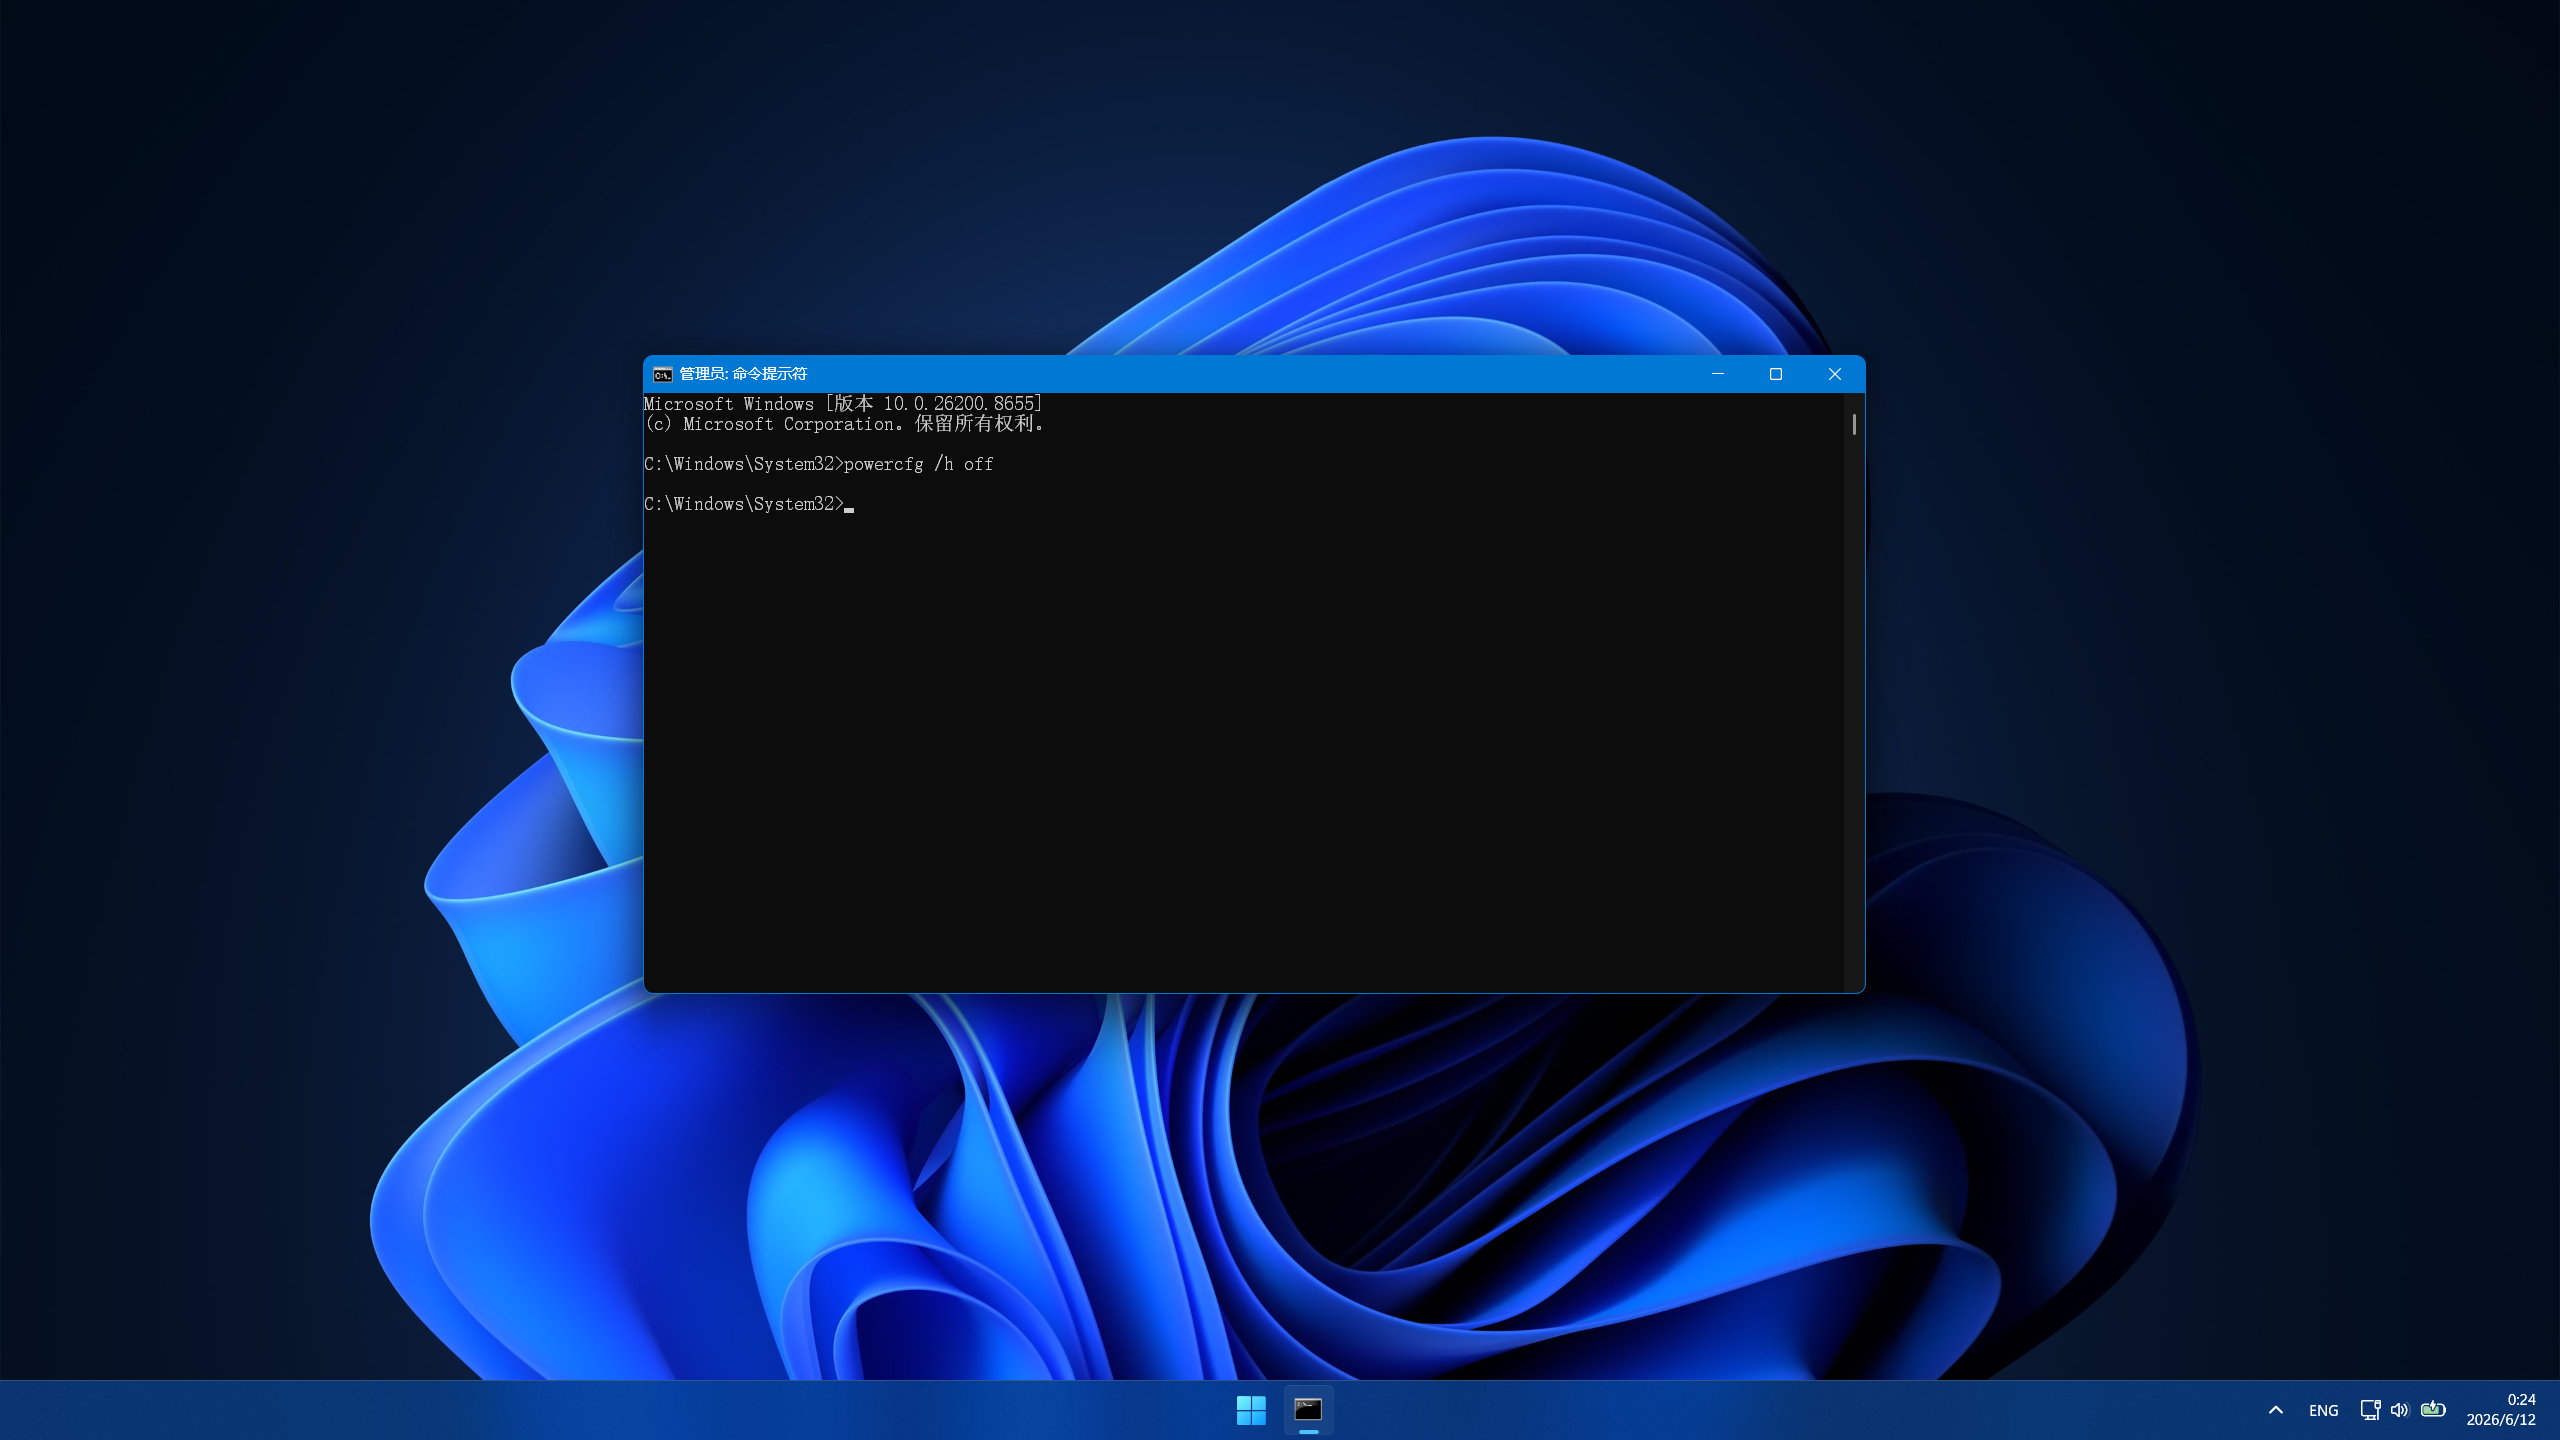
\includegraphics[width=0.8\textwidth]{10.png} 
\end{figure}
\newpage
\subsection{关闭安全启动}
接下来我们要进入电脑的BIOS设置界面，关闭安全启动。不同品牌的电脑进入BIOS的方式和BIOS的界面均有所不同，以下以我的联想拯救者R9000P为例。
\smallbreak
先关机电脑，等待电脑完全关机后，按下电源键开机，然后马上按住 \keys{F2} 键不放，直到进入BIOS界面。
\smallbreak
以下是我的BIOS界面
\begin{figure}[H]
    \centering 
    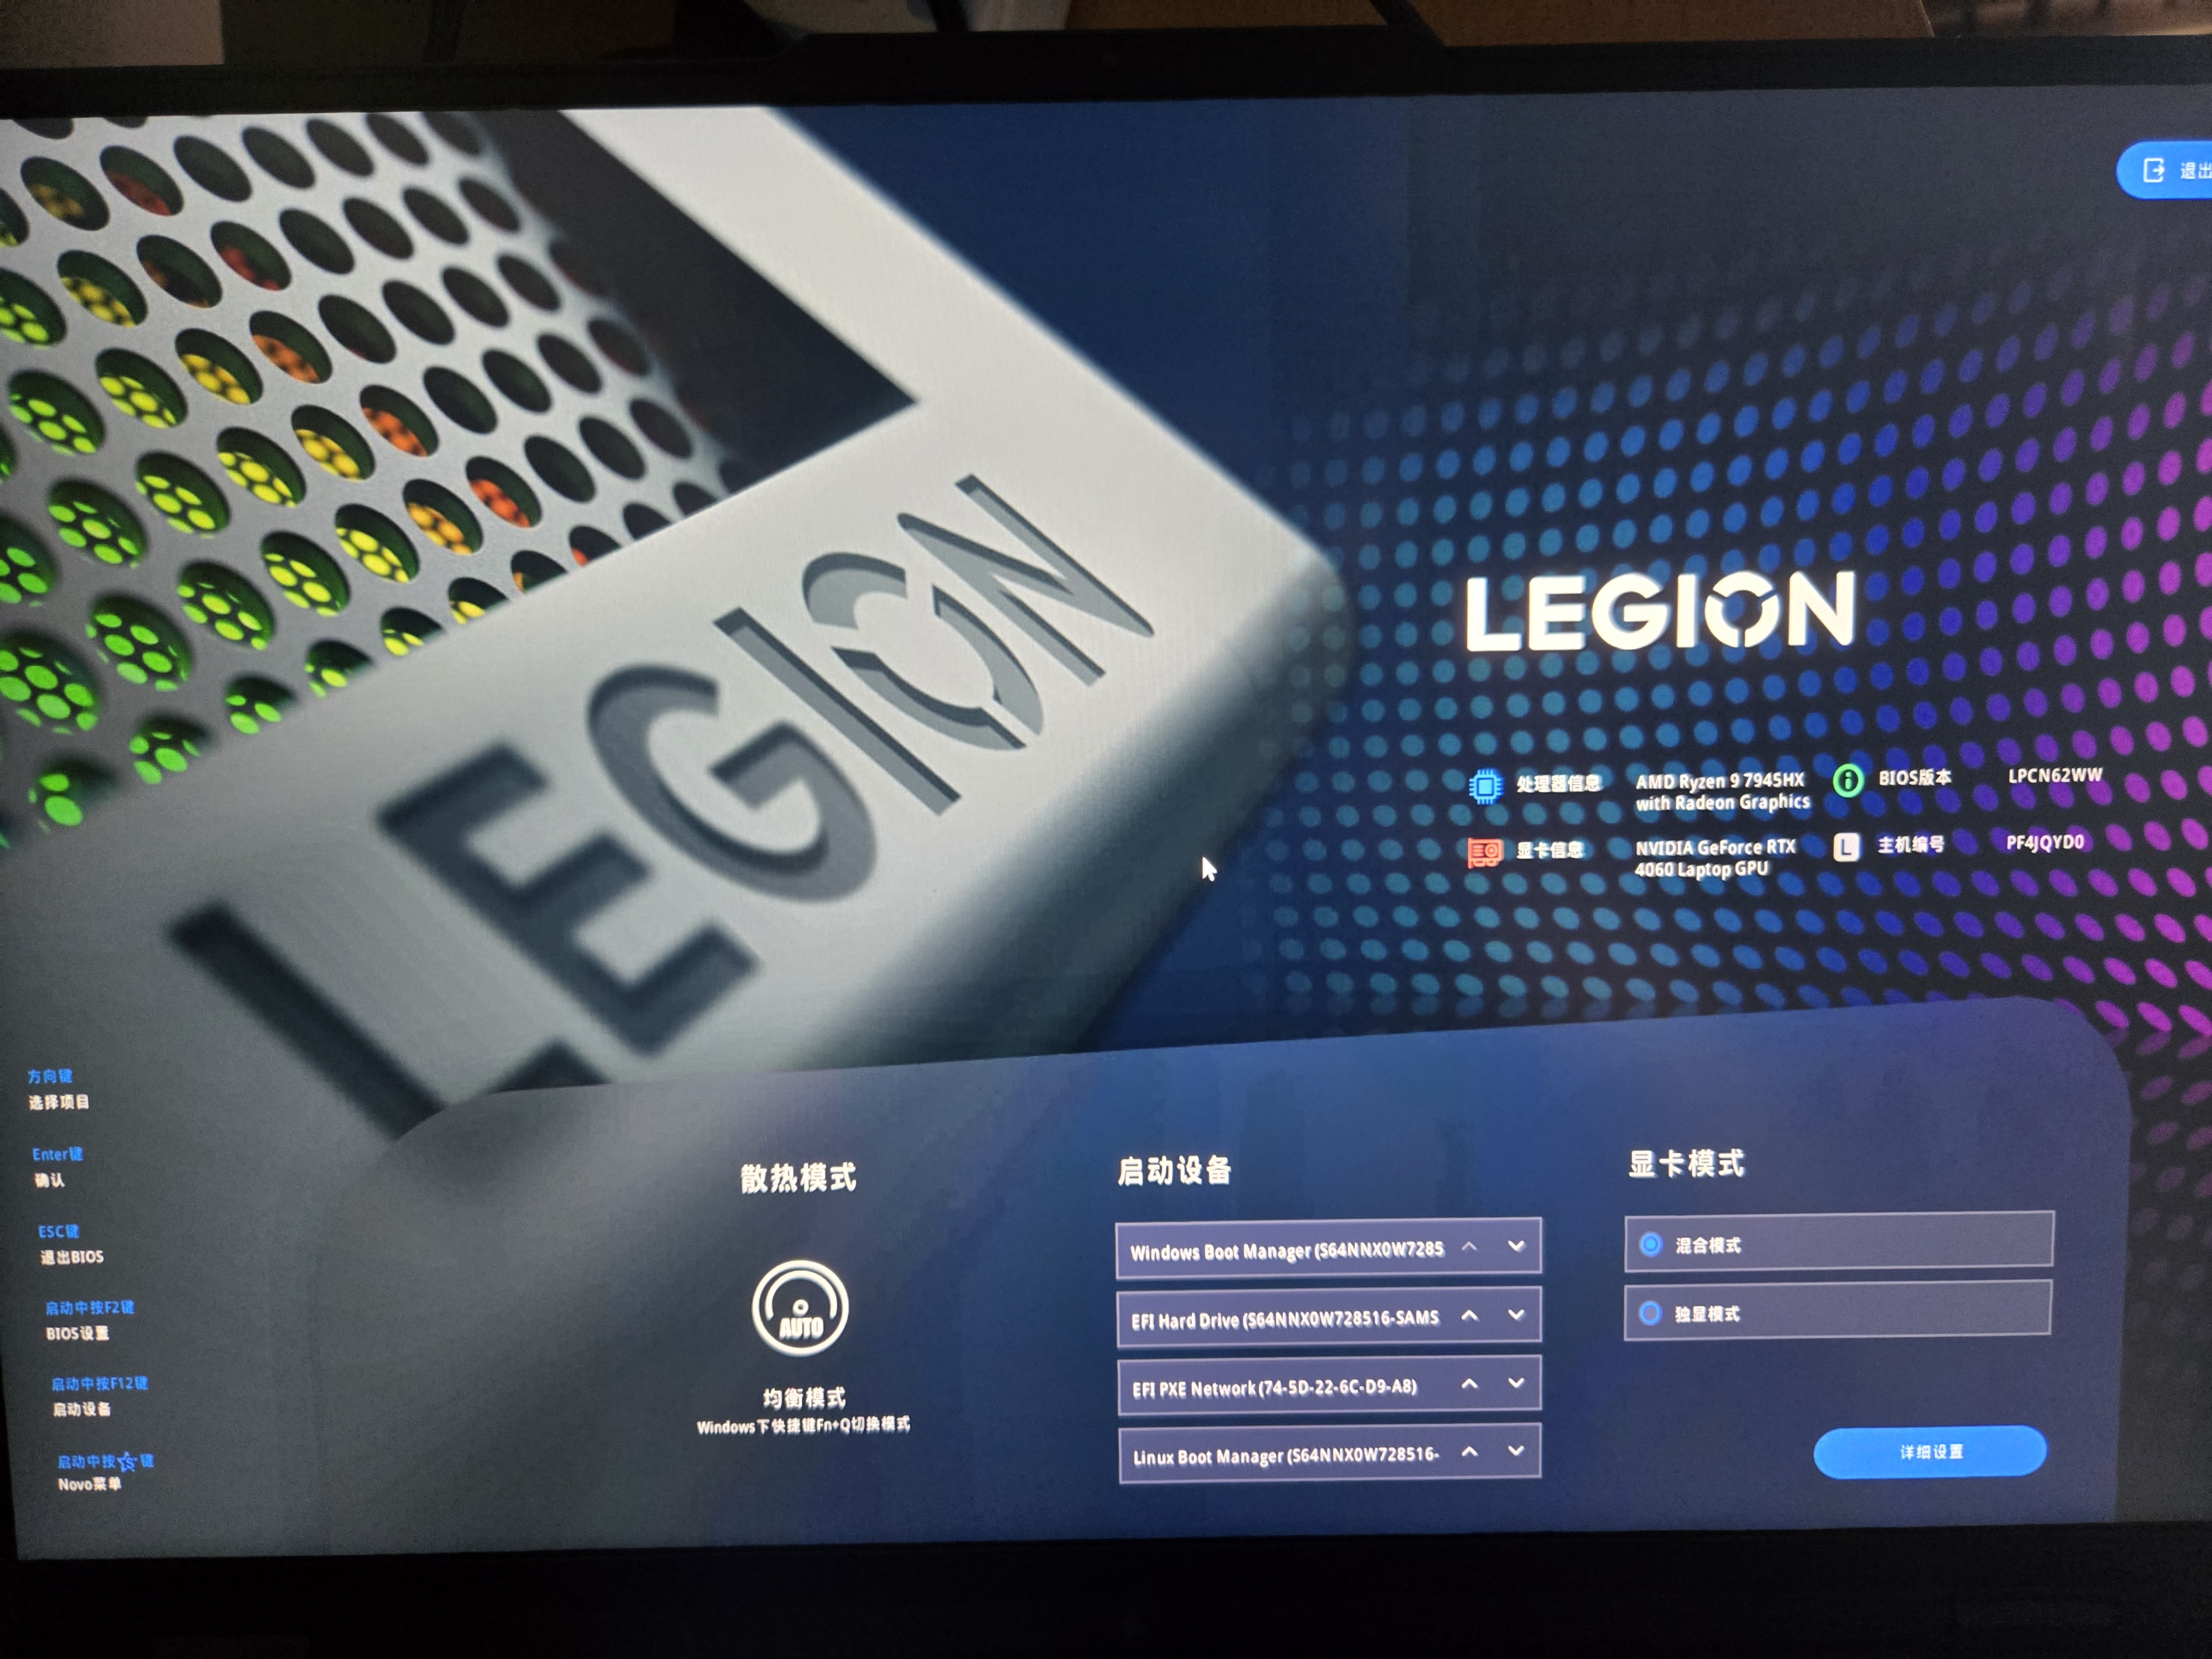
\includegraphics[width=0.65\textwidth]{bios.jpg} 
\end{figure}
如果有独立显卡的，需要把独显模式改成混合模式，安装完成后可以再改回独显模式。
\smallbreak
然后点击\textbf{详细设置}，在\textbf{安全设置}里找到\textbf{安全启动}，选择\textbf{关闭}。其他品牌电脑可以自己找一下。
\smallbreak
改好设置后，按下 \keys{F10} 保存并退出BIOS设置界面，然后电脑会重启，在重启的过程中按住 \keys{F12} 进入启动菜单，然后看本教程下一节的内容。
\begin{figure}[H]
    \centering 
    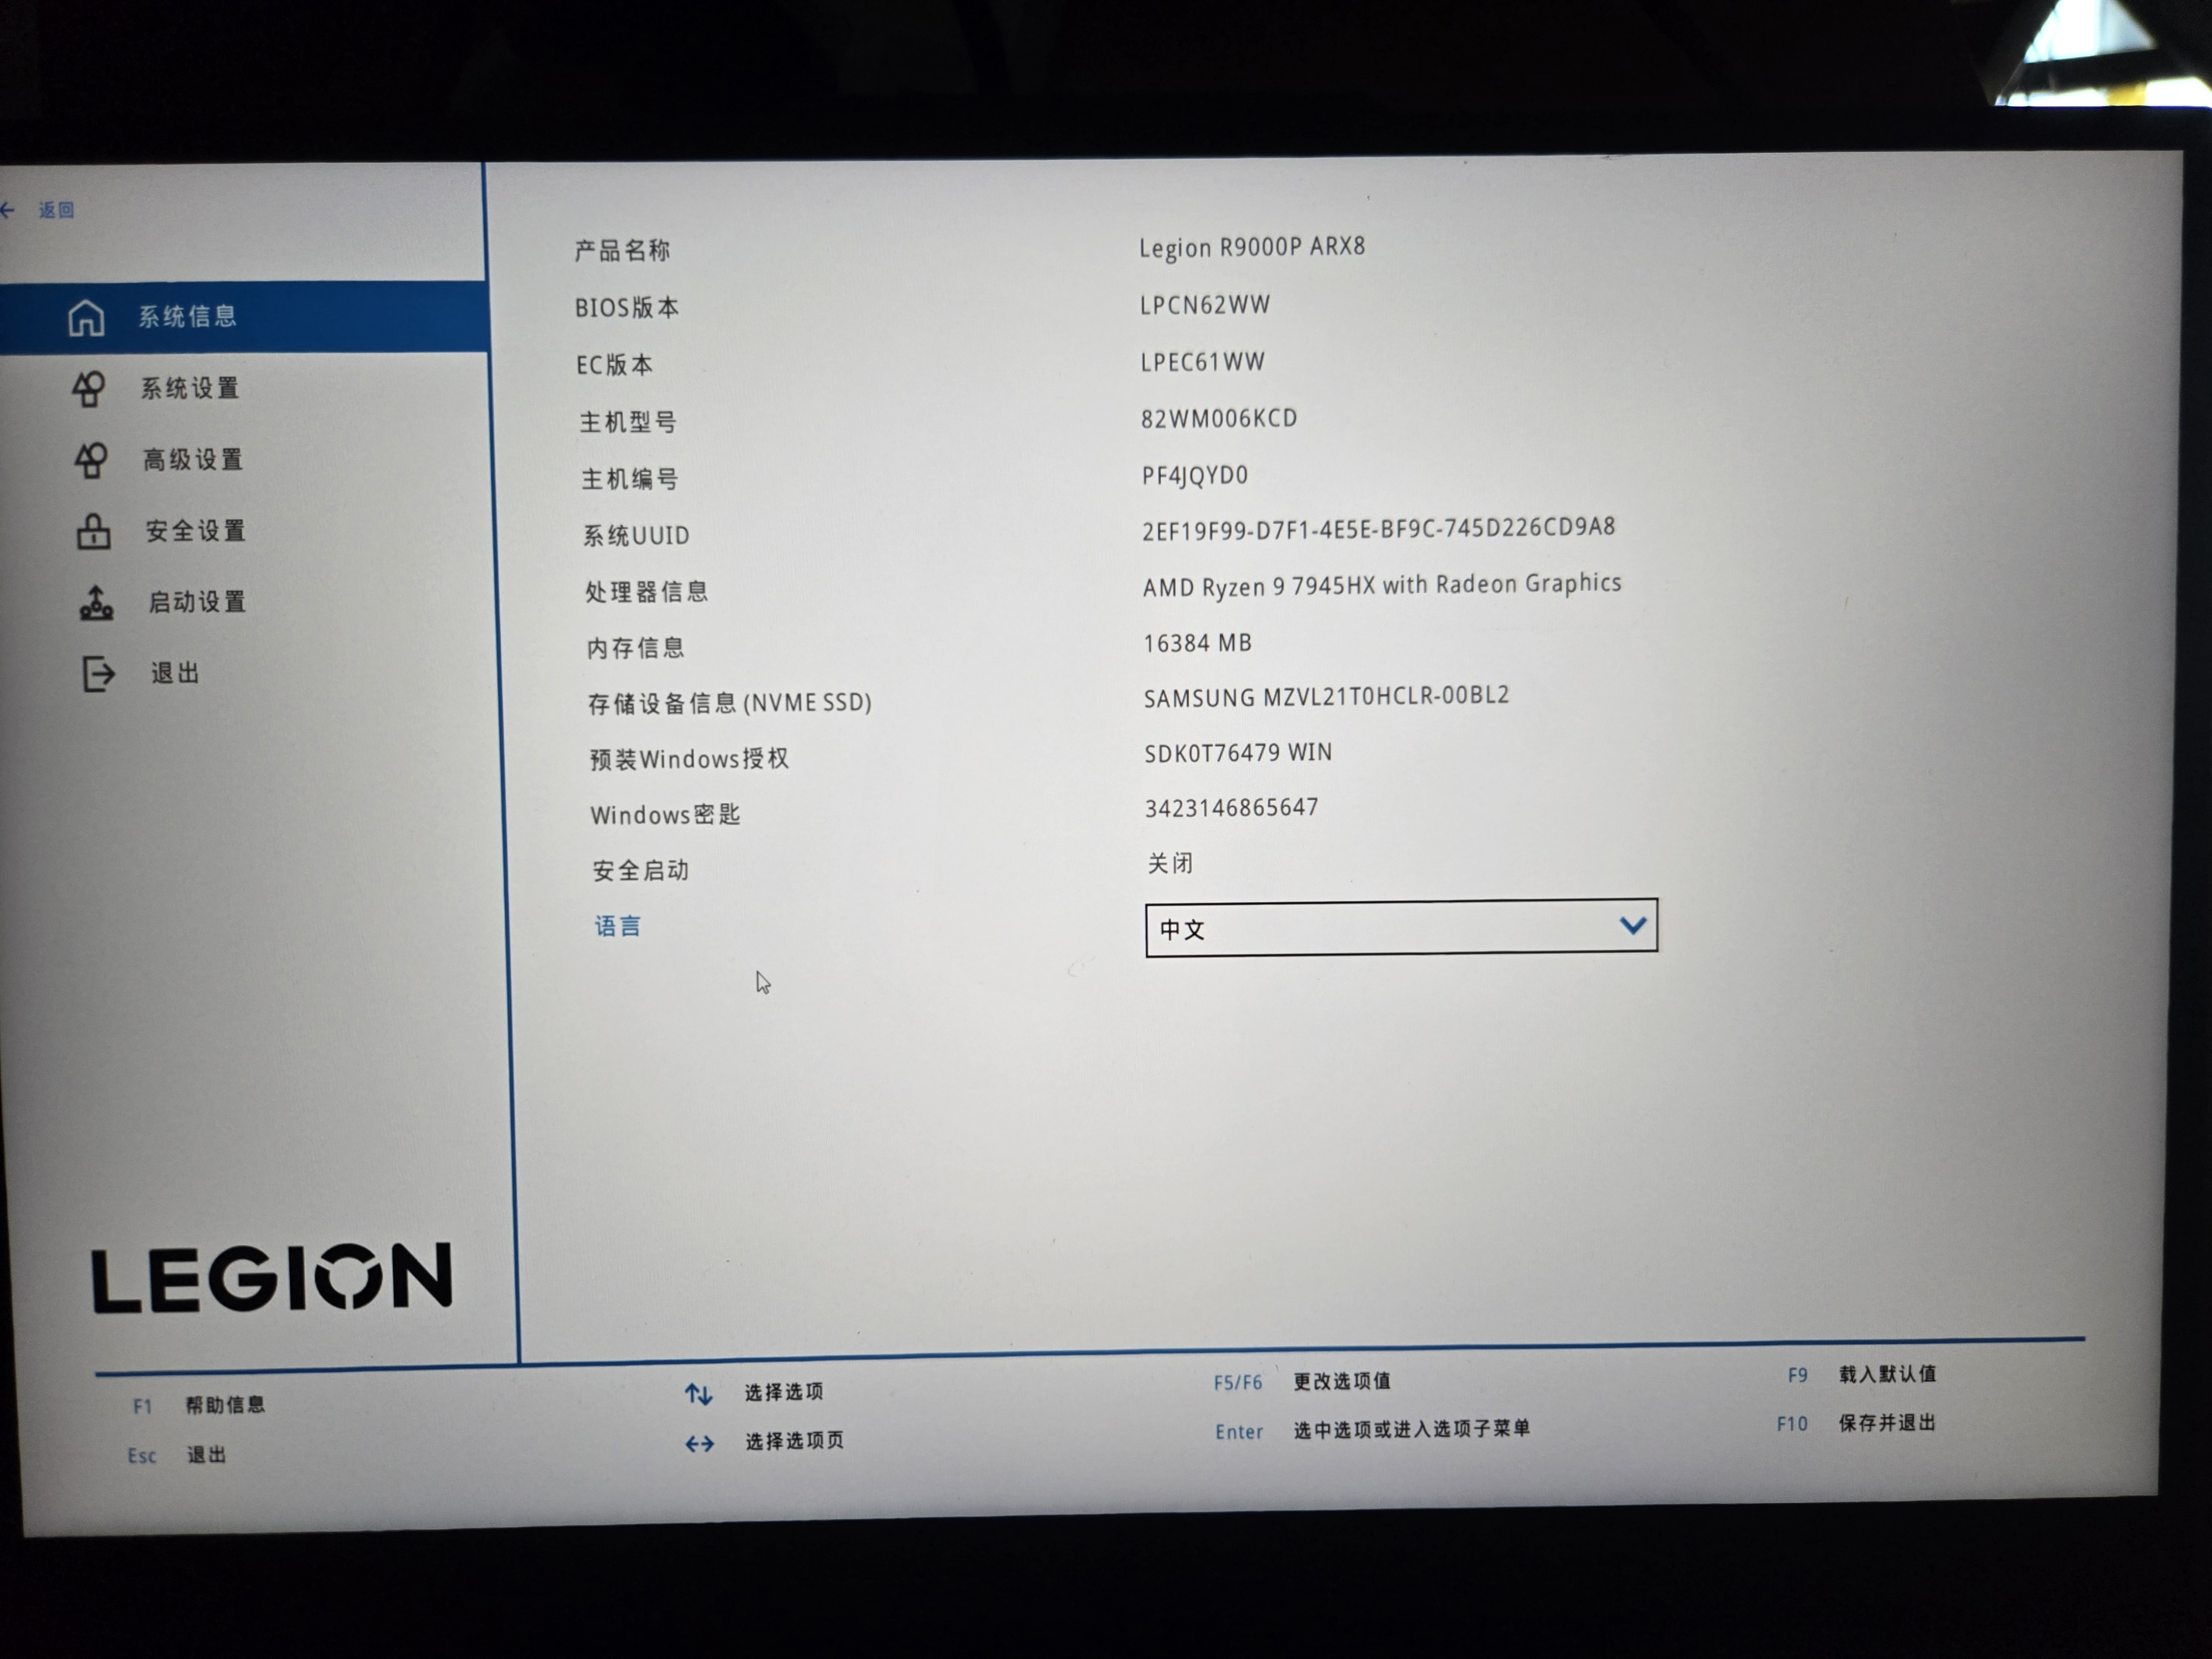
\includegraphics[width=0.65\textwidth]{bios2.jpg} 
\end{figure}
\section{安装Ubuntu} 
在电脑启动的过程中按住 \keys{F12} 进入启动菜单，选择从U盘启动。如下图，第五个选项就是我的U盘了，鼠标点它，或者用方向键选中它后按回车。
\begin{figure}[H]
    \centering 
    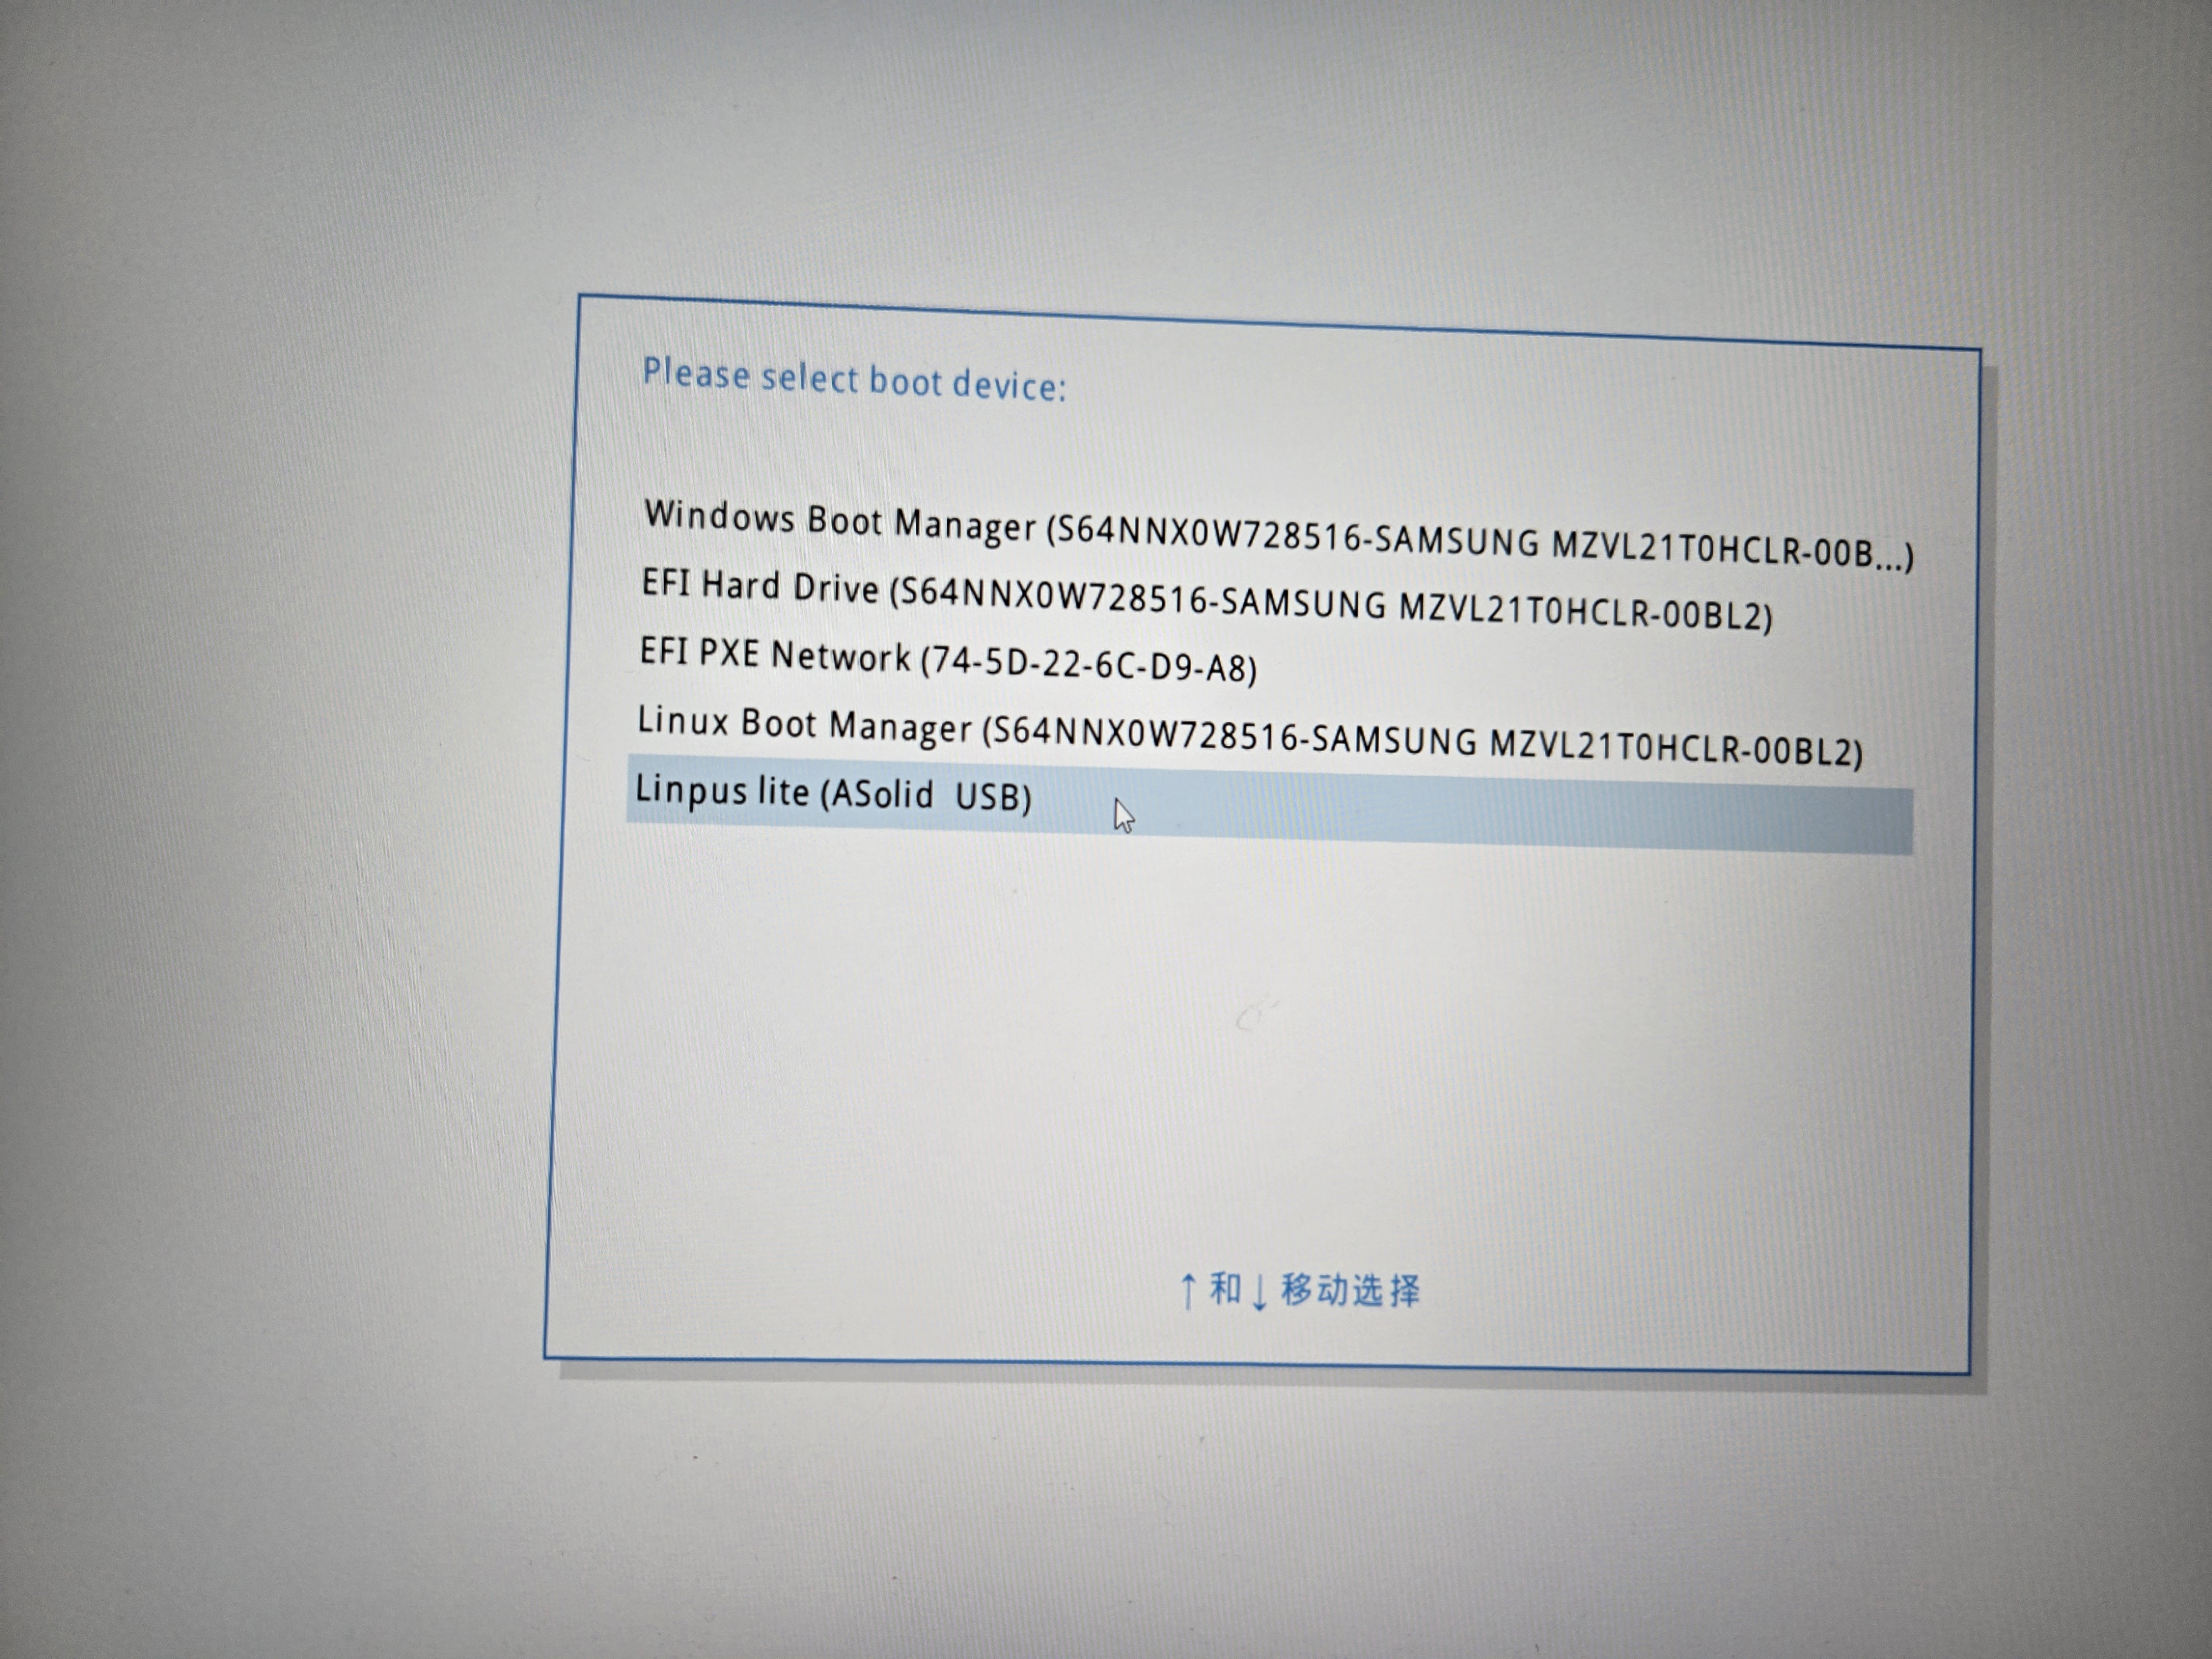
\includegraphics[width=0.7\textwidth]{boot_menu2.jpg} 
\end{figure}
然后会出来一个选择界面，选择第一个选项“Try or Install Ubuntu”。
\begin{figure}[H]
    \centering 
    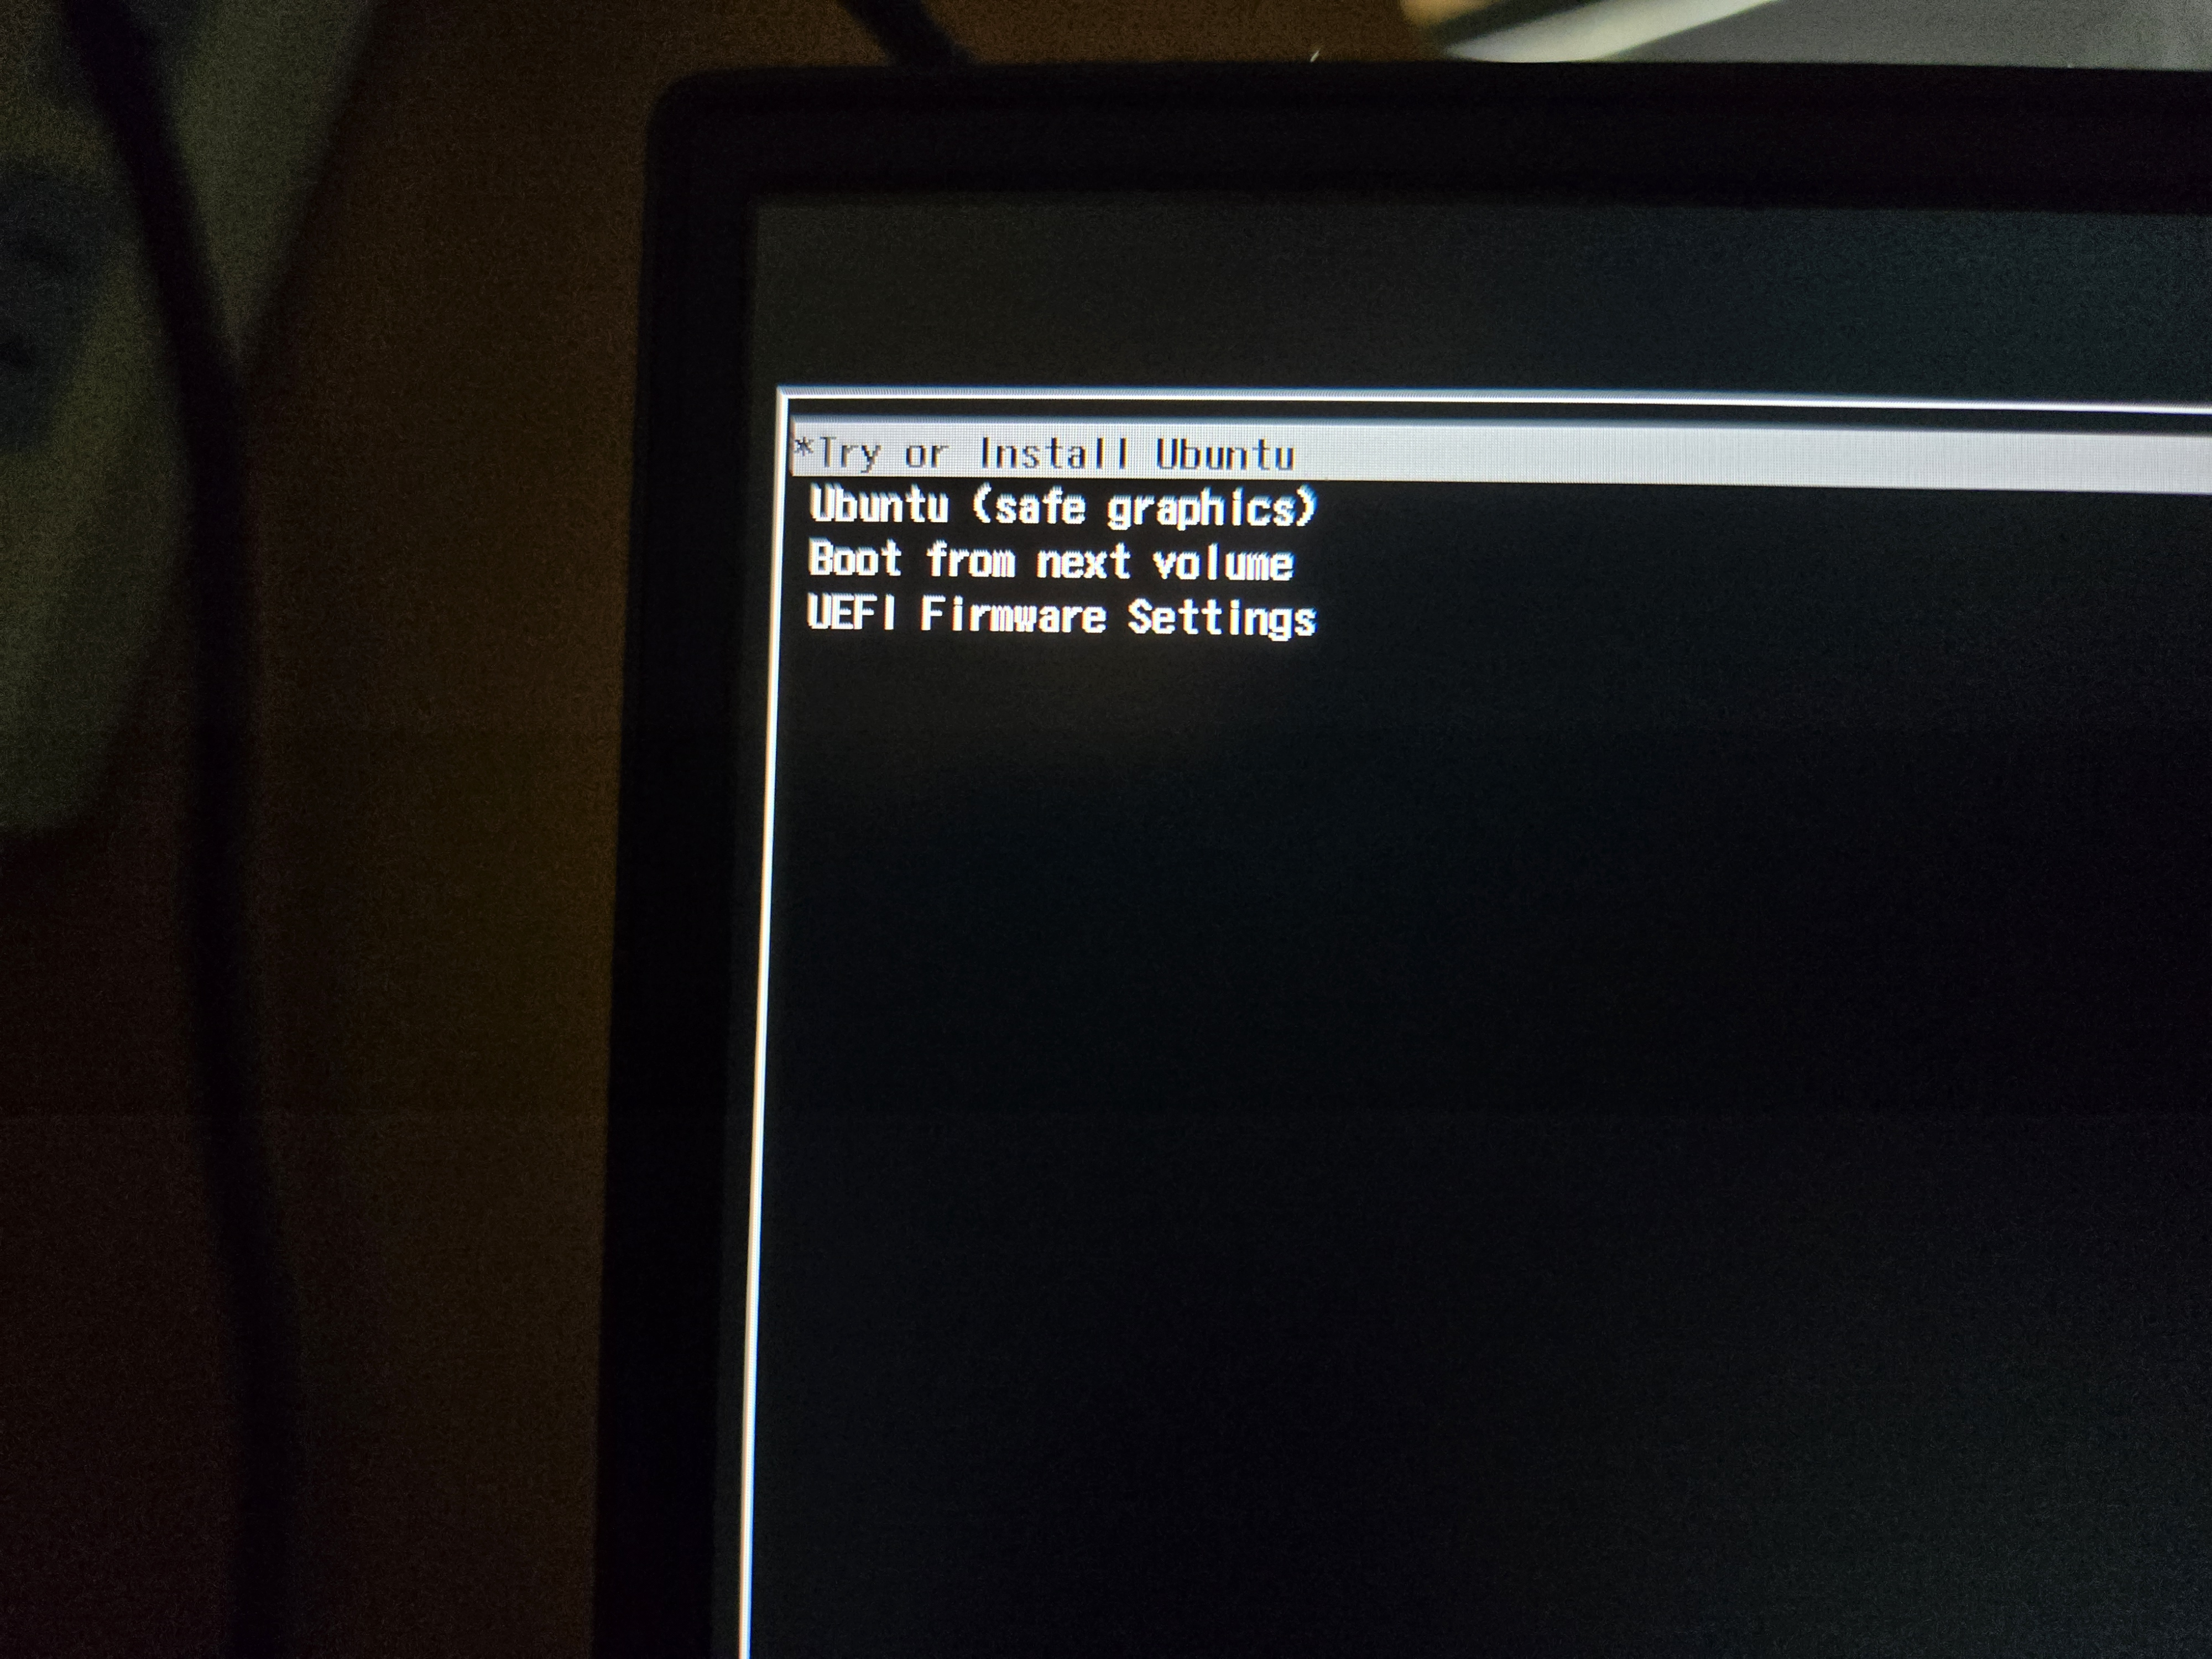
\includegraphics[width=0.7\textwidth]{ubuntu.jpg} 
\end{figure}
然后我们就进入了Ubuntu的试用界面了，接下会弹出安装向导，如果没有弹出安装向导，就点击桌面上的\textbf{install Ubuntu 24.04.4 LTS}，如果出现问题了可以多重启几次电脑试试。
\smallbreak
最后跟着向导完成安装即可，安装过程中会有一些选项需要选择，以下是一些截图供参考。
\begin{figure}[H]
    \centering 
    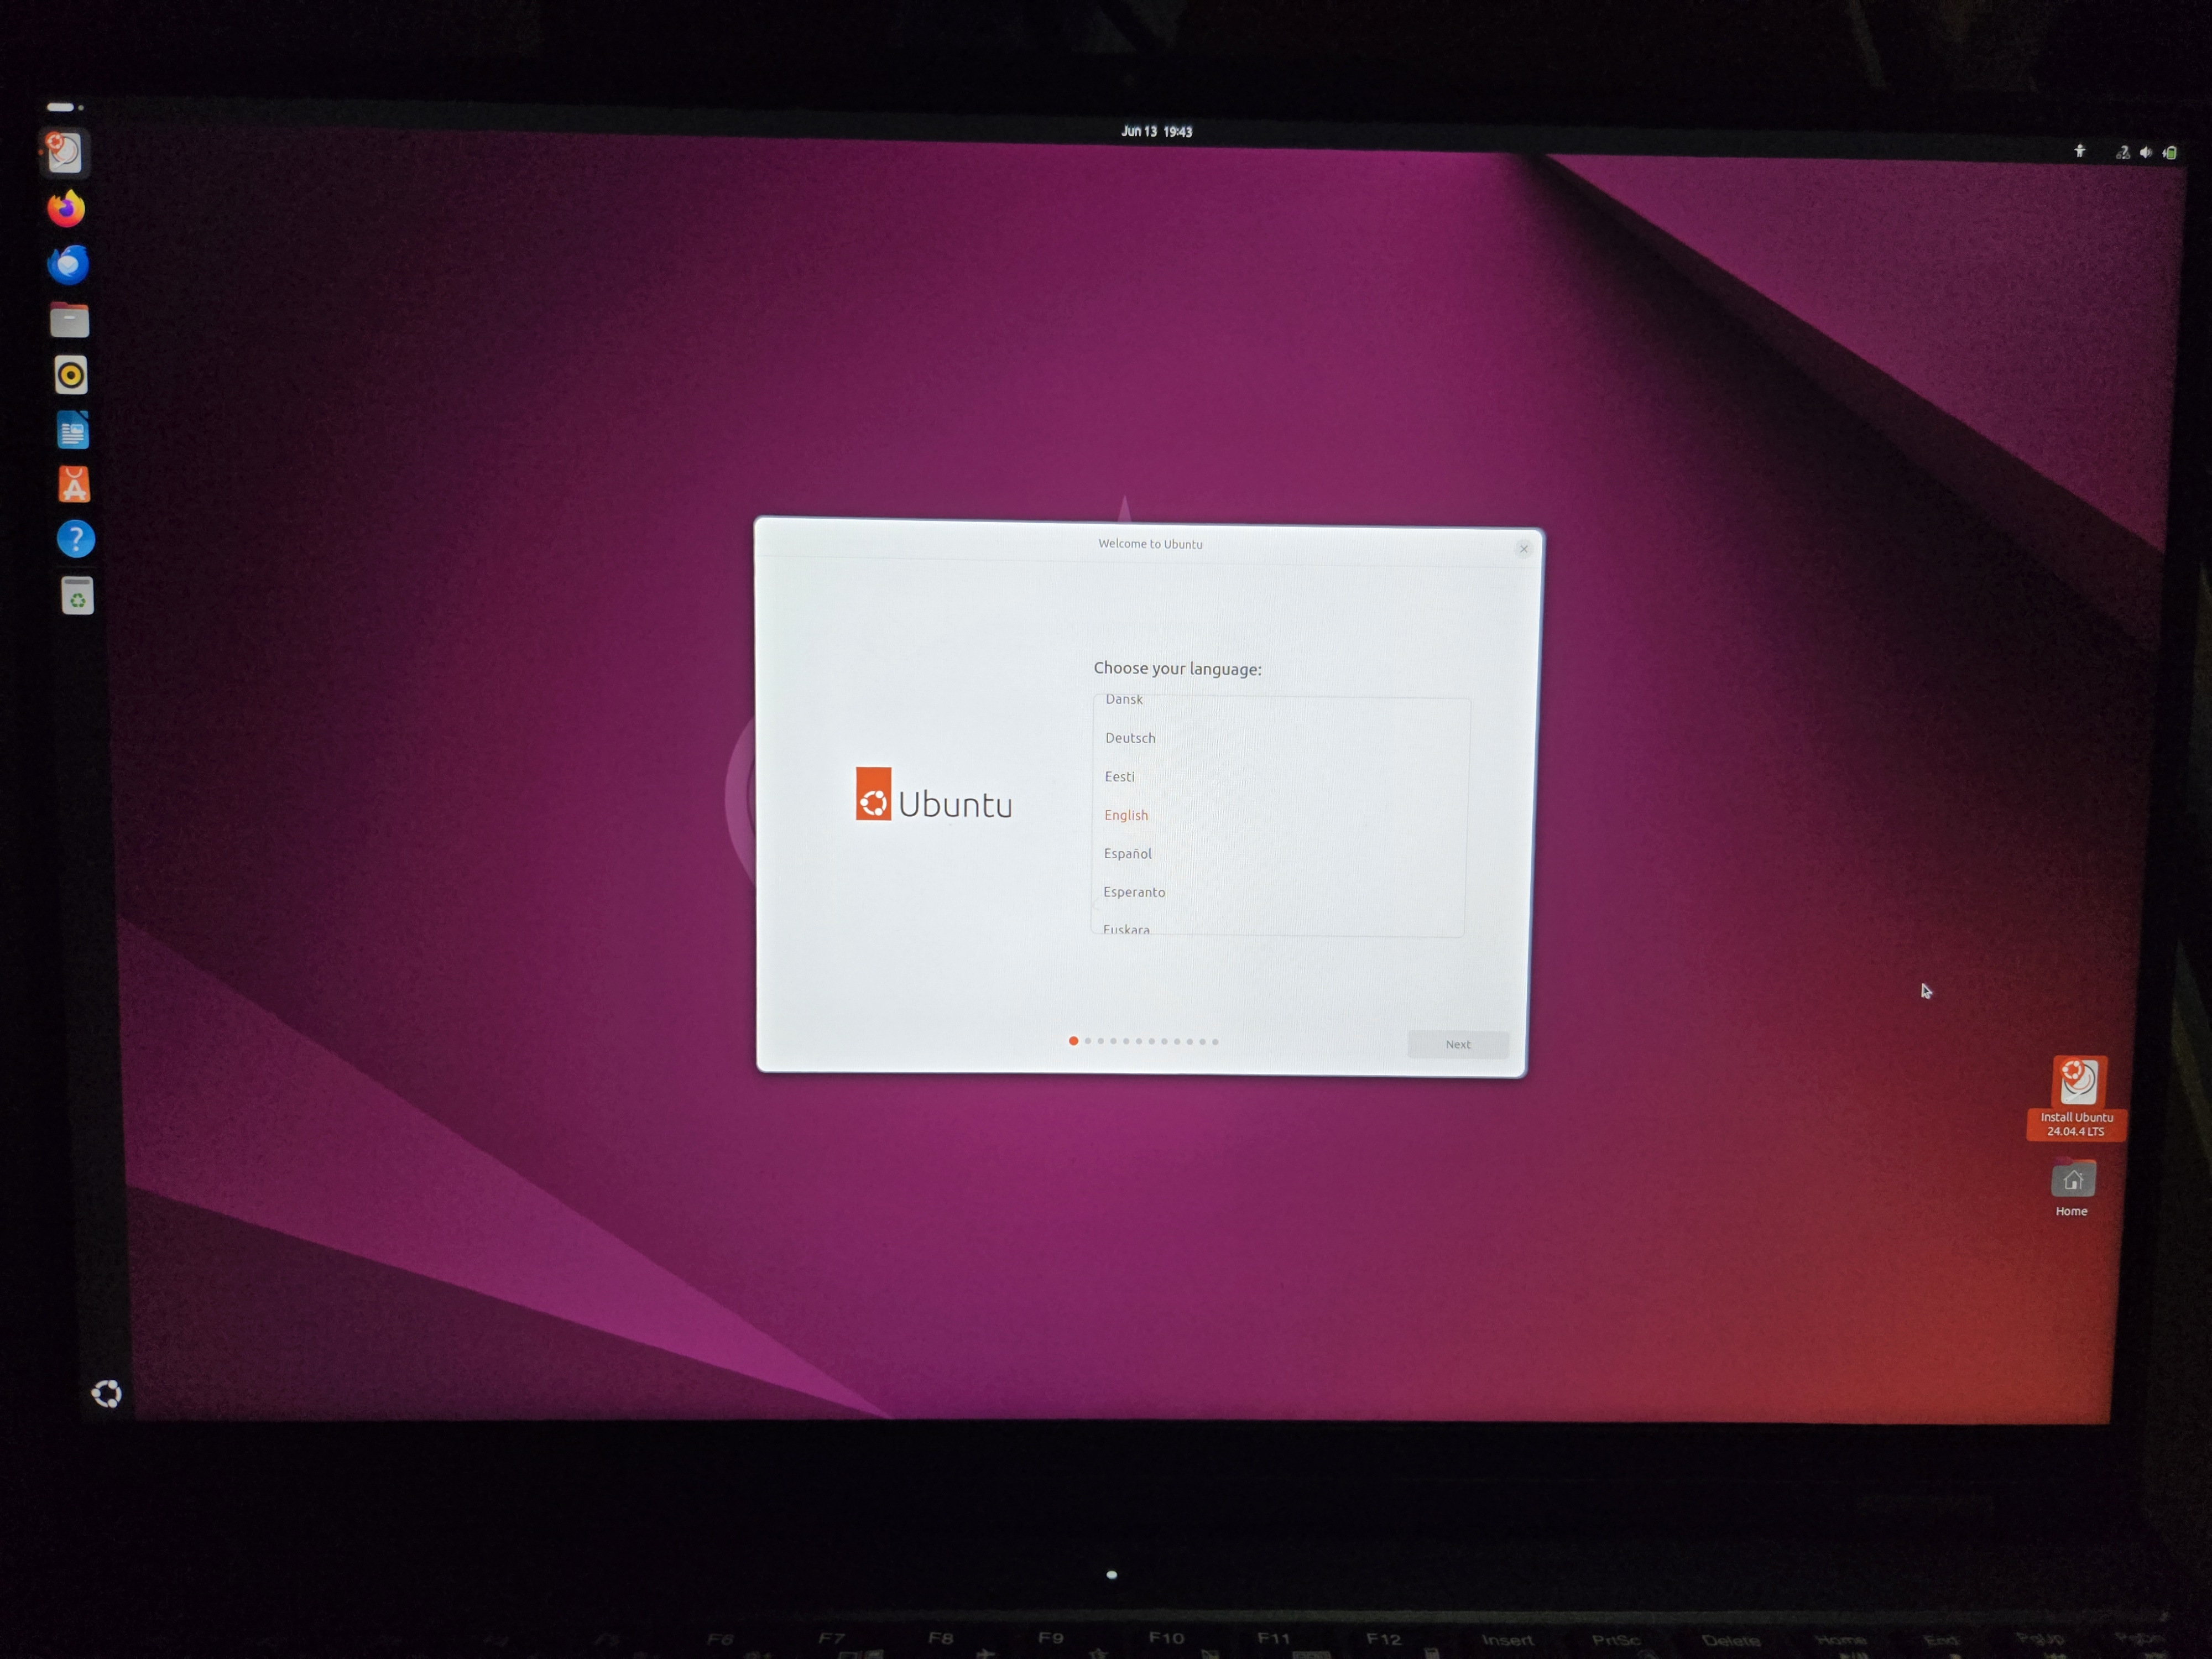
\includegraphics[width=0.8\textwidth]{ubuntu2.jpg} 
\end{figure}
\begin{figure}[H]
    \centering 
    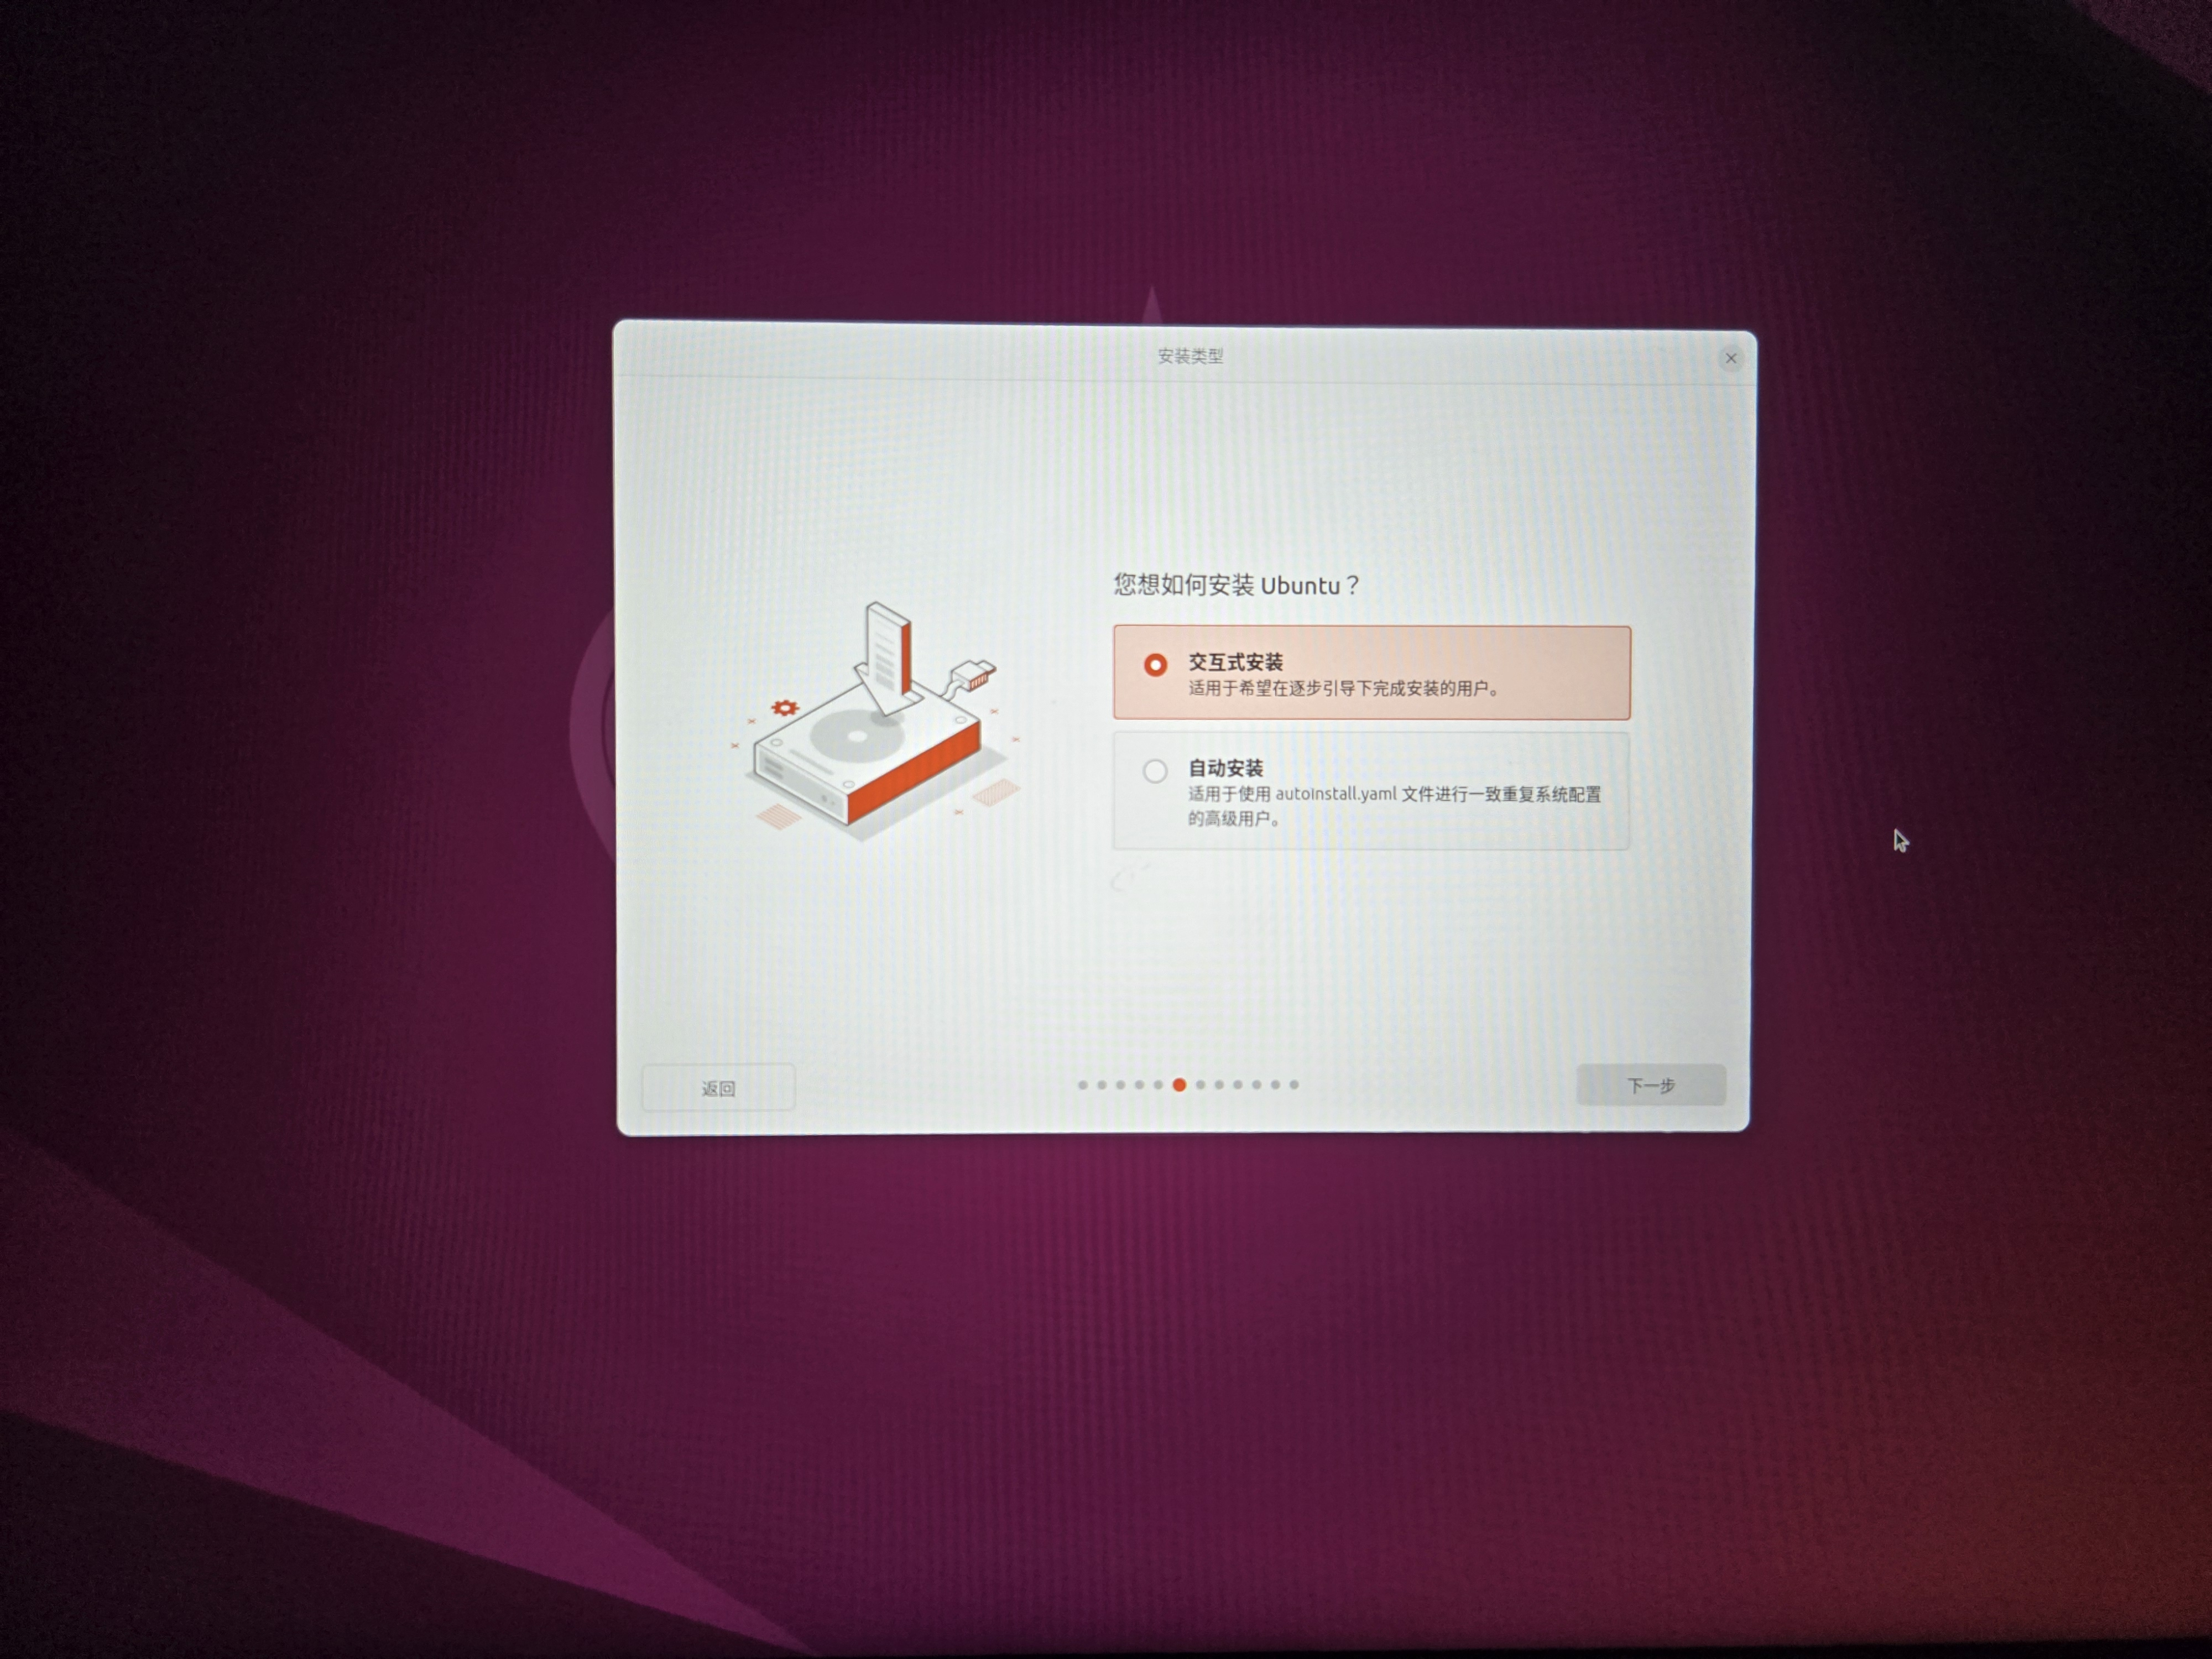
\includegraphics[width=0.8\textwidth]{ubuntu3.jpg} 
\end{figure}
\begin{figure}[H]
    \centering 
    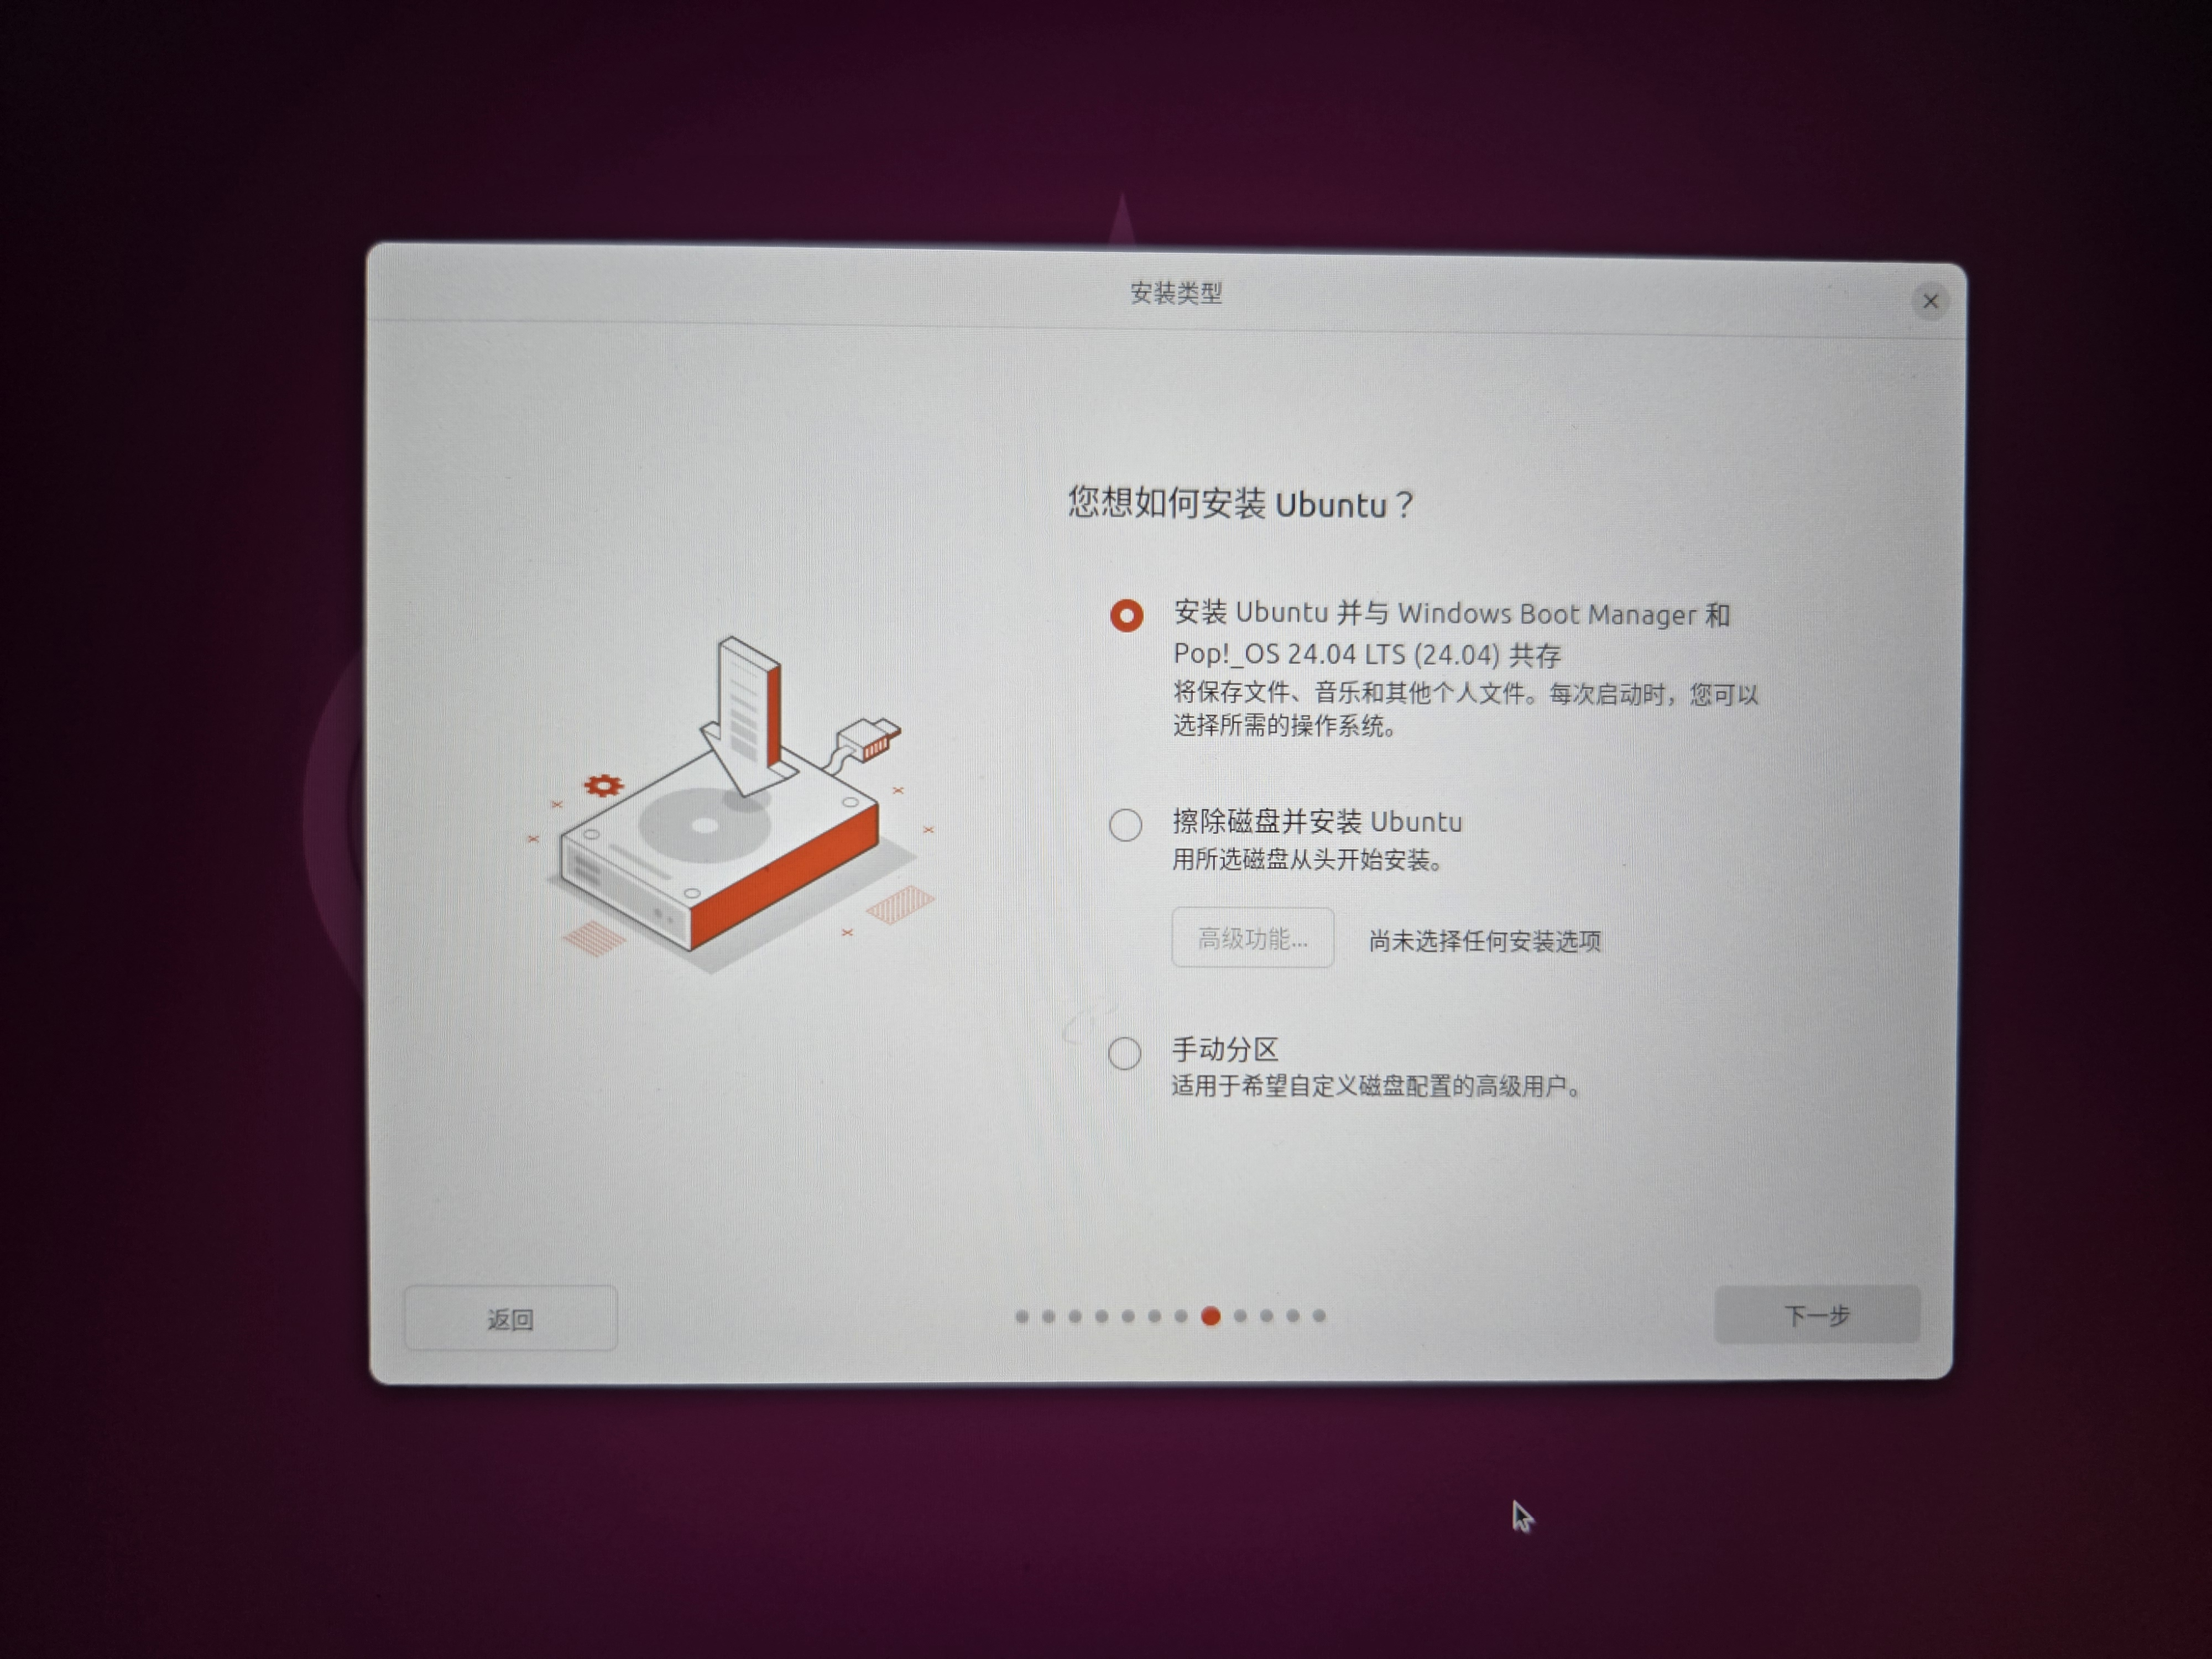
\includegraphics[width=0.8\textwidth]{ubuntu4.jpg} 
\end{figure}
\begin{figure}[H]
    \centering 
    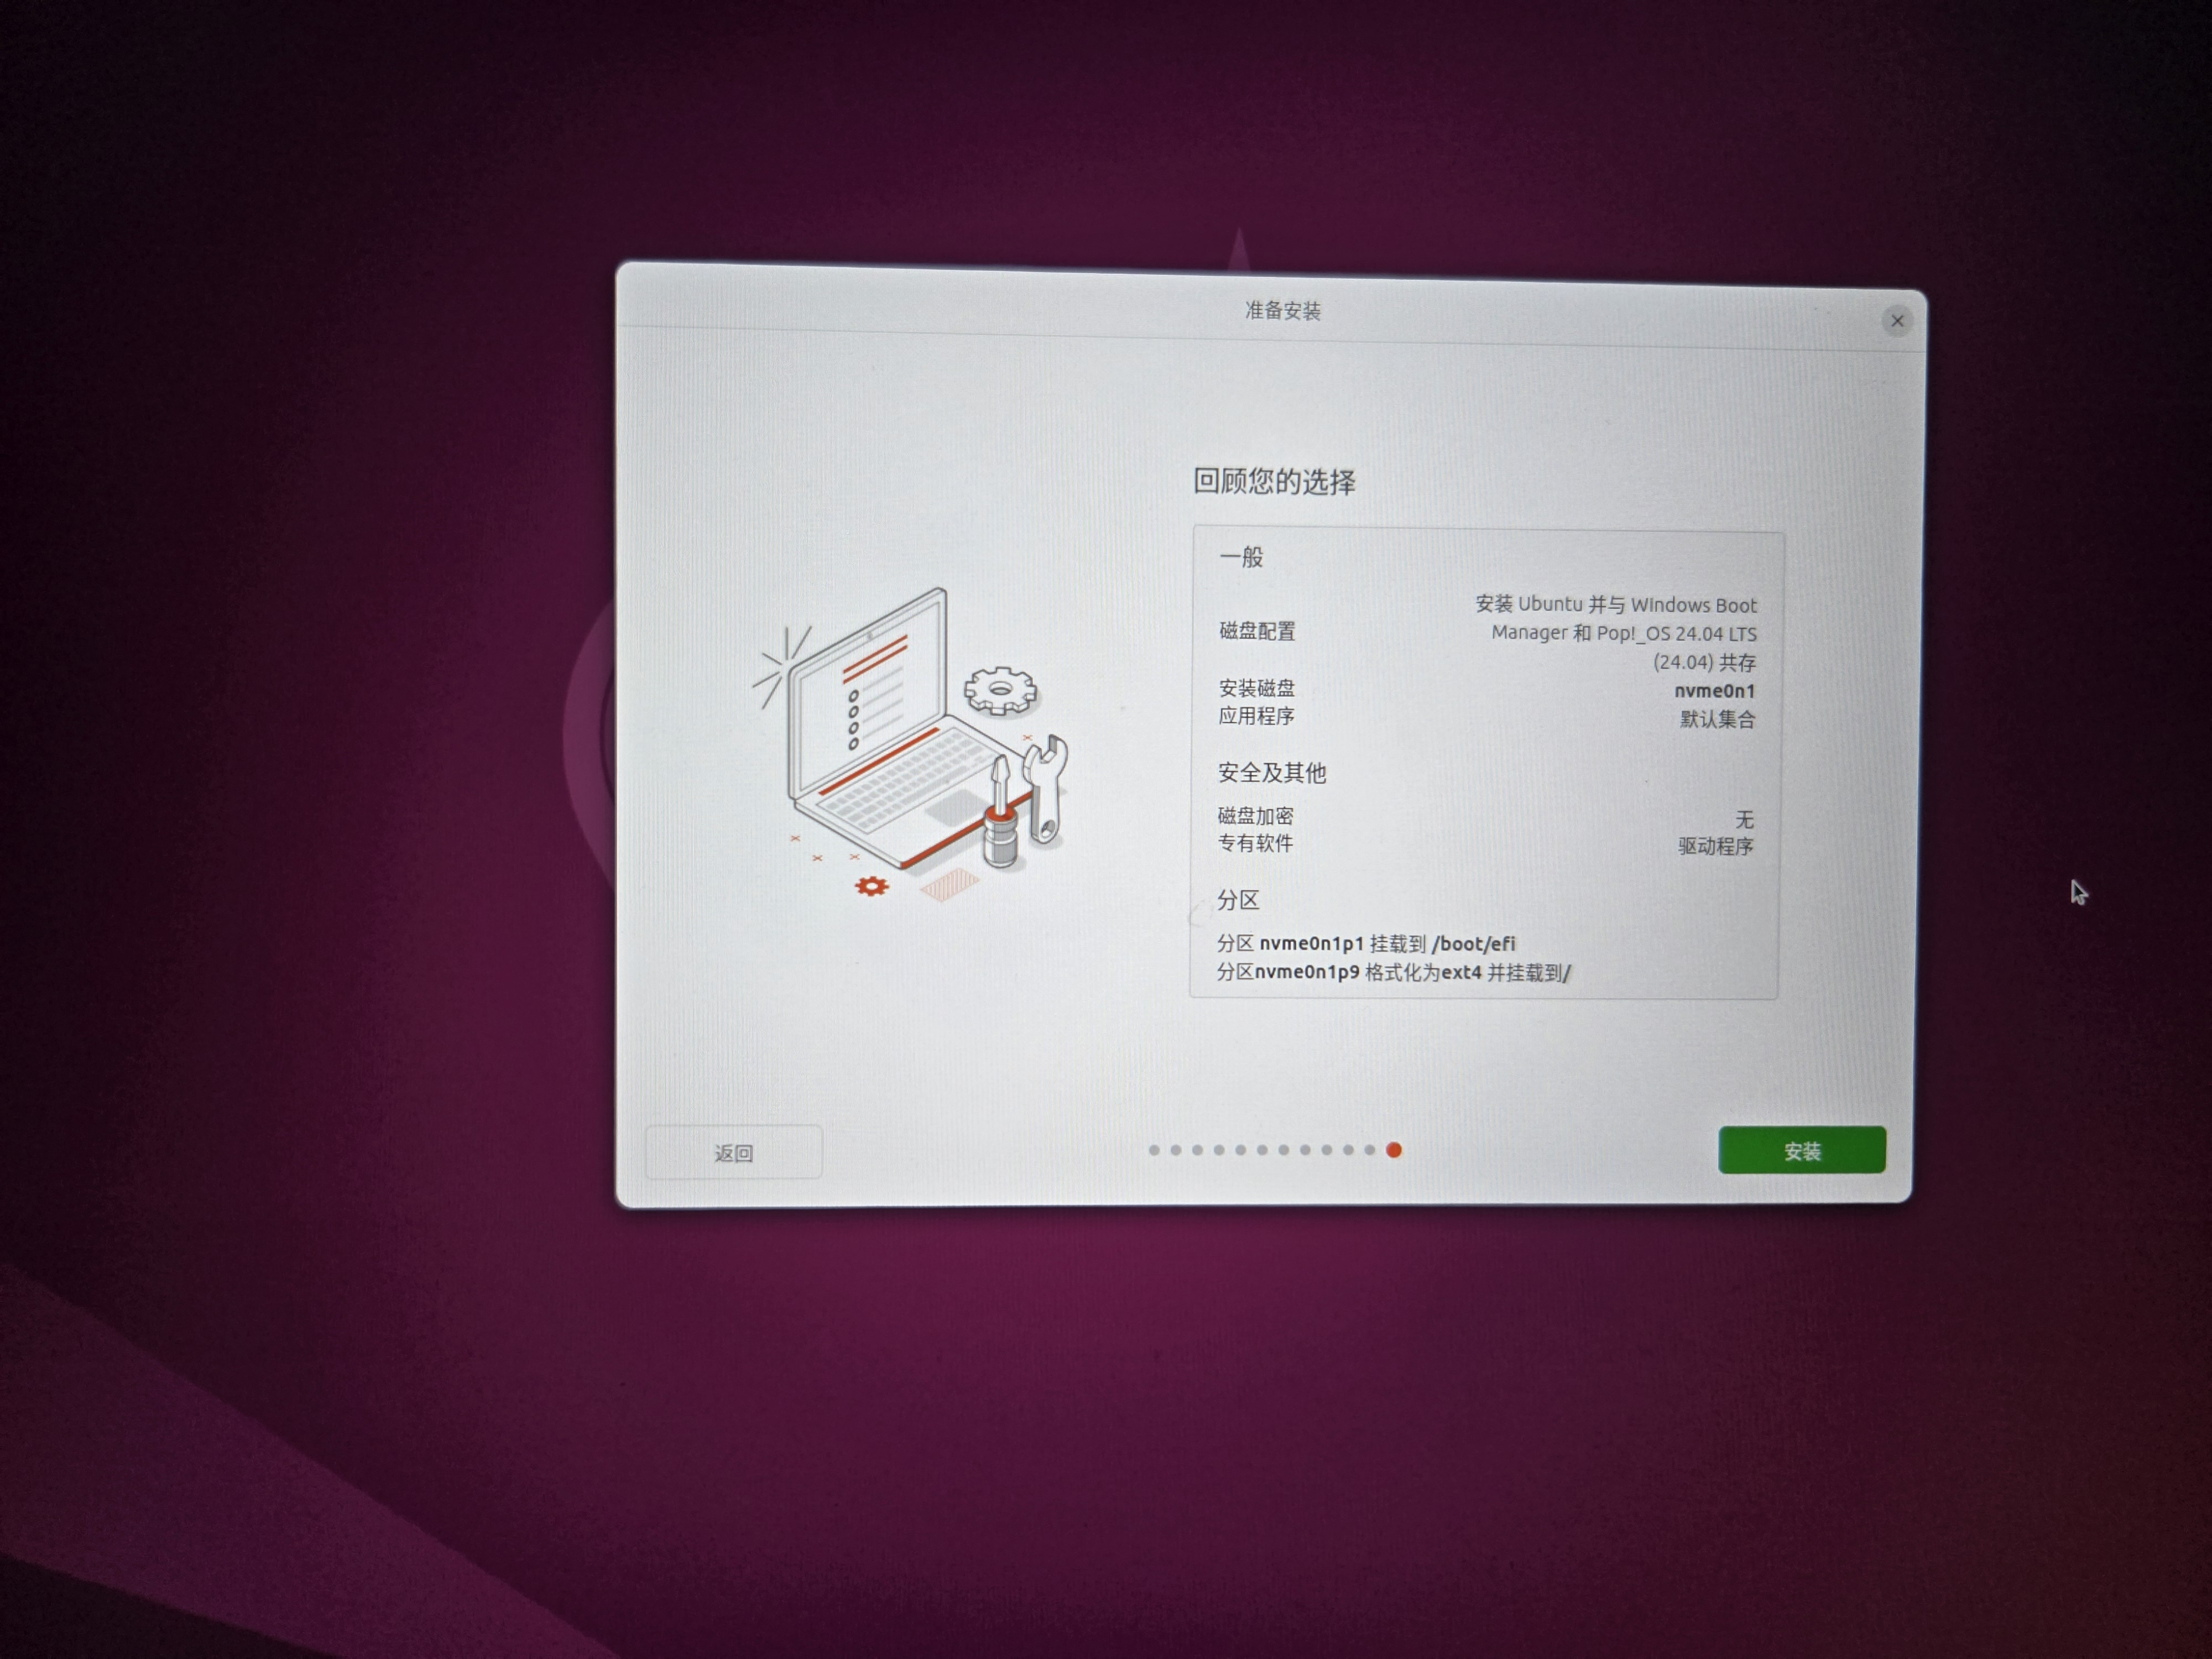
\includegraphics[width=0.8\textwidth]{ubuntu5.jpg} 
\end{figure}

\end{document}
